\documentclass[10pt]{memoir}
\setstocksize{220mm}{155mm} 	        
\settrimmedsize{220mm}{155mm}{*}	
\settypeblocksize{170mm}{116mm}{*}	
\setlrmargins{18mm}{*}{*}
\setulmargins{*}{*}{1.2}
%\setlength{\headheight}{5pt}%
\checkandfixthelayout[lines]
\linespread{1.16}
\flushbottom

%%% Hyphenation settings
\usepackage[htt]{hyphenat}
\hyphenation{he-lio-trope opos-sum}
\tracingparagraphs=1
%Hyphenation in Devanāgarī of the edition still missing? Probably this needs to be modified in babel-iast package? 

%%% babel
\usepackage[english]{babel}
\usepackage{babel-iast/babel-iast}

\babelfont[iast]{rm}[Renderer=Harfbuzz, Scale=1.3]{AdishilaSan}%AdishilaSan}
\babelfont[english]{rm}{Adobe Text Pro}

%%% more functionality
\PassOptionsToPackage{hyphens}{url}
\usepackage{hyperref}
\usepackage{pdflscape}
\usepackage{cleveref}
\usepackage{url}
\usepackage{cleveref}
\usepackage{microtype}
\usepackage{lineno}

%\usepackage{bigfoot}
%%% more functions
\usepackage[dvipsnames]{xcolor}
%\usepackage[para,perpage]{footmisc}

%%%für den Counter von Kapiteln und Sätzen! 
\newcommand{\uproman}[1]{\uppercase\expandafter{\romannumeral#1}}
\newcommand{\lowroman}[1]{\romannumeral#1\relax}

\makeindex
\newfontfamily\sanskritfont[Script=Devanagari,Mapping=RomDev,Scale=1.1]{Sanskrit2003}
\usepackage{pifont,fourier-orns,lettrine,psvectorian,paralist,enumitem,pdfpages,wrapfig,tabulary,lettrine,longtable}
\setlist[enumerate]{itemsep=0mm}
\usepackage[autostyle]{csquotes}
\usepackage[defaultlines=2,all]{nowidow}
\usepackage{ellipsis,adforn,booktabs,longtable,url,tikz}
\lineskiplimit=-3pt          

\makechapterstyle{IeT}{%
  \chapterstyle{default}
  \renewcommand*{\printchapternonum}{\centering}
  \renewcommand*{\clearforchapter}{\cleartorecto} 
  \aliaspagestyle{chapter}{empty}}
\chapterstyle{IeT}
\setsecnumdepth{none}  \openright  \nouppercaseheads
\settocdepth{subsubsection}

%%%% test better pagebreaks
%\def\fussy{%
%  \emergencystretch\z@
%  \tolerance 200%
%  \hfuzz .1\p@
%  \vfuzz\hfuzz}

%\interfootnotelinepenalty=10000\relax

%\usepackage[maxfloats=256]{morefloats}

%\maxdeadcycles=500

%raggedbottomsectiontrue
%%\checkandfixthelayout


%%%%%%%  biblatex
%\newcommand{\noun}[1]{\textsc{#1}}    %  philosophy-verbose
\usepackage[backend=biber, sorting=nyt, style=verbose]{biblatex} %%%%ORIGINAL TiE
\renewcommand*{\mkbibnamefamily}[1]{\textsc{#1}}


\DeclareFieldFormat{url}{%
  \mkbibacro{URL}\addcolon\space
  \href{#1}{\nolinkurl{\thefield{urlraw}}}}

\DeclareFieldFormat{citeurl}{%
  \href{#1}{\nolinkurl{\thefield{urlraw}}}} 


\DeclareFieldFormat{postnote}{#1}
\renewcommand{\postnotedelim}{, }
\addbibresource{bindu.bib}

%%% ekdosis
\usepackage[teiexport=tidy,parnotes=true]{ekdosis}% =tidy cleans up HTML and XML documents by fixing markup errors and upgrading legacy code to modern standards. parnotes=footnotes below or above critical apparatus

\SetLineation{lineation=page, modulo} %lineation=page sets thenumbering to start afresh at the top of each page. =modulo makes every fifth line numbered. {lineation=page} makes every line numbered! 

\renewcommand{\linenumberfont}{\selectlanguage{english}\footnotesize} %sets language of lines to English

\SetTEIxmlExport{autopar=false} %autopar=falseinstructs ekdosis to ignore blank lines in the.tex sourcefile as markers for paragraph boundaries. As a result, each paragraph of the edition must be found within an environment associated with the xml <p> element

\SetHooks{
  lemmastyle=\bfseries,
  %refnumstyle=\selectlanguage{english}\bfseries,
  refnumstyle=\selectlanguage{english}\color{blue}\bfseries,
  appheight=0.8\textheight,
}

\newif\ifinapparatus
\DeclareApparatus{source}[
%bhook=\inapparatustrue,
lang=english,
notelang=english,
% bhook=\selectlanguage{english},
bhook=\selectlanguage{english}\textbf{Sources:},%
%maxentries=4, 
%ehook=.]
%sep={] },
%nosep,
]

\newif\ifinapparatus
\DeclareApparatus{testium}[
%bhook=\inapparatustrue,
lang=english,
notelang=english,
% bhook=\selectlanguage{english},
bhook=\selectlanguage{english}\textbf{Testimonia:},
%maxentries=4, 
%ehook=.]
%nosep, 
]

% Declare \ifinapparatus and set \inapparatustrue at the beginning of
% the apparatus criticus block. Also set the language.  
\newif\ifinapparatus
  \DeclareApparatus{default}[
  %bhook=\inapparatustrue, 
  lang=english,
  %maxentries=33,
  %bhook=\selectlanguage{english},
  sep = {] },
  delim=\hskip 0.75em,
  rule=\rule{0.7in}{0.4pt},
]

\newif\ifinapparatus
\DeclareApparatus{philcomm}[
%bhook=\inapparatustrue,
lang=english,
notelang=english,
bhook=\selectlanguage{english}\textbf{Philological Commentary:},
%bhook=\selectlanguage{english},
sep={: },
]

\ekdsetup{
showpagebreaks,
spbmk = \textcolor{blue}{spb},
hpbmk = \textcolor{red}{hpb}
}

%\usepackage{fnpos}
%\makeFNmid
%\makeFNbottom
\usepackage[bottom]{footmisc}
%%%%%%%%%%%%%%%%%%%%%%%%%%%
\makeatletter
\def\blfootnote{\gdef\@thefnmark{}\@footnotetext}
\makeatother
%%%%%%%%%%%%%%%%%%%%%%%%%


% Macros and Definitions for the Print of Sigla
\def\acpc#1#2#3{{#1}\rlap{\textrm{\textsuperscript{#3}}}\textsubscript{\textrm{#2}}\space}
\def\sigl#1#2{{{#1}}\textsubscript{\textrm{#2}}}
\def\None{{\sigl{N}{1}}} \def\Noneac{\acpc{N}{1}{ac}\,} \def\Nonepc{\acpc{N}{1}{pc}\,}
\def\Ntwo{{\sigl{N}{2}}} \def\Noneac{\acpc{N}{2}{ac}\,} \def\Nonepc{\acpc{N}{2}{pc}\,}
\def\Done{{\sigl{D}{1}}} \def\Doneac{\acpc{D}{1}{ac}\,} \def\Donepc{\acpc{D}{1}{pc}\,}
\def\Dtwo{{\sigl{D}{2}}} \def\Dtwoac{\acpc{D}{2}{ac}\,} \def\Dtwopc{\acpc{D}{2}{pc}\,}
\def\Uone{{\sigl{U}{1}}} \def\Uoneac{\acpc{U}{1}{ac}\,} \def\Uonepc{\acpc{U}{1}{pc}\,}                 
\def\Utwo{{\sigl{U}{2}}} \def\Utwoac{\acpc{U}{2}{ac}\,} \def\Utwopc{\acpc{U}{2}{pc}\,}

%%%%%%%%%%%%%% Tattvabinduyoga - List of Witnesses   %%%%%%%%%%%%%%%%%%%
\DeclareWitness{ceteri}{\selectlanguage{english}cett.}{ceteri}[]   
\DeclareWitness{E}{\selectlanguage{english}E}{Printed Edition}[]    
\DeclareWitness{P}{\selectlanguage{english}P}{Pune BORI 664}[]  
\DeclareWitness{B}{\selectlanguage{english}B}{Bodleian 485}[]       
\DeclareWitness{N1}{\selectlanguage{english}N\textsubscript{1}}{NGMPP 38/31}[]
\DeclareWitness{N2}{\selectlanguage{english}N\textsubscript{2}}{NGMPP B 38/35}[]
\DeclareWitness{L}{\selectlanguage{english}L}{LALCHAND 5876}[]  
\DeclareWitness{D}{\selectlanguage{english}D}{IGNCA 30019}[] 
%\DeclareWitness{D2}{\selectlanguage{english}D\textsubscript{2}}{IGNCA 30020}[]  
\DeclareWitness{U1}{\selectlanguage{english}U\textsubscript{1}}{SORI 1574}[] 
\DeclareWitness{U2}{\selectlanguage{english}U\textsubscript{2}}{SORI 6082}[]
%%%%%%%%%%%%%% Tattvabinduyoga - Groups of Witnesses   %%%%%%%%%%%%%%%%%%%
\DeclareWitness{X}{\selectlanguage{english}\alpha}{Alpha Group: D,N1,N2,U1}[]
\DeclareWitness{Y}{\selectlanguage{english}\beta}{Beta Group: B,E,L,P,U2}[]
%%%%%%%%%%%%% Testimonia
\DeclareWitness{Ysv}{\selectlanguage{english}Ysv}{Yogasvarodaya}[] %%%add infos!  

%%%%%%%%%%%%%%%%%%%%%%%%%%%%%%%%%%%%%%%%%%%
% Macro for Editing Abbrevs.
\def\om{\textrm{\footnotesize \textit{om.}\ }} %prints om. for omitted in apparatus
\def\korr{\textrm{\footnotesize \textit{em.}\ }} %prints em. for emended in apparatus
\def\conj{\textrm{\footnotesize \textit{conj.}\ }} %prints conj. for conjectured in apparatus

% \supplied{text} EDITORIAL ADDITION -> Within \lem oder \rdg
% \surplus{text} EDITORIAL DELETION -> Within \lem oder \rdg
% \sic{text} CRUX
% \gap{text} LACUNAE -> [reason=??, unit=??, quantity=??, extent=??]


%%%%%%%%%%%%%%%%%%%%%%%%%%%%%%%%%%%%%%%%%%% All macros of this list can be used in 
% Macro for Editing Abbrevs.
\def\eyeskip{\textrm{{ab.\,oc. }}}
\def\aberratio{\textrm{{ab.\,oc. }}}
\def\ad{\textrm{{ad}}}
\def\add{\textrm{{add.\ }}}
\def\ann{\textrm{{ann.\ }}}
\def\ante{\textrm{{ante }}} 
\def\post{\textrm{{post }}}
%\def\ceteri{cett.\,}                   
\def\codd{\textrm{{codd.\ }}}

\def\coni{\textrm{{coni.\ }}}
\def\contin{\textrm{{contin.\ }}}
\def\corr{\textrm{{corr.\ }}}
\def\del{\textrm{{del.\ }}}
\def\dub{\textrm{{ dub.\ }}}

\def\expl{\textrm{{explic.\ }}} 
\def\explica t{\textrm{{explic.\ }}}
\def\fol{\textrm{{fol.\ }}}
\def\foll{\textrm{{foll.\ }}}
\def\gloss{\textrm{{glossa ad }}}
\def\ins{\textrm{{ins.\ }}}      
\def\inseruit{\textrm{{ins.\ }}} 
\def\im{{\kern-.7pt\lower-1ex\hbox{\textrm{\tiny{\emph{i.m.}}}\kern0pt}}} %\textrm{\scriptsize{i.m.\ }}}      
\def\inmargine{{\kern-.7pt\lower-.7ex\hbox{\textrm{\tiny{\emph{i.m.}}}\kern0pt}}}%\textrm{\scriptsize{i.m.\ }}}      
\def\intextu{{\kern-.7pt\lower-.95ex\hbox{\textrm{\tiny{\emph{i.t.}}}\kern0pt}}}%\textrm{\scriptsize{i.t.\ }}}           
\def\indist{\textrm{{indis.\ }}}  
\def\indis{\textrm{{indis.\ }}}
\def\iteravit{\textrm{{iter.\ }}} 
\def\iter{\textrm{{iter.\ }}}
\def\lectio{\textrm{{lect.\ }}}   
\def\lec{\textrm{{lect.\ }}}
\def\leginequit{\textrm{{l.n. }}} 
\def\legn{\textrm{{l.n. }}}
\def\illeg{\textrm{{l.n. }}}

\def\primman{\textrm{{pr.m.}}}
\def\prob{\textrm{{prob.}}}
\def\rep{\textrm{{repetitio }}}
\def\secundamanu{\textrm{\scriptsize{s.m.}}}            \def\secm{{\kern-.6pt\lower-.91ex\hbox{\textrm{\tiny{\emph{s.m.}}}\kern0pt}}}%   \textrm{\scriptsize{s.m.}}}
\def\sequentia{\textrm{{seq.\,inv.\ }}}  
\def\seqinv{\textrm{{seq.\,inv.\ }}}
\def\order{\textrm{{seq.\,inv.\ }}}
\def\supralineam{{\kern-.7pt\lower-.91ex\hbox{\textrm{\tiny{\emph{s.l.}}}\kern0pt}}} %\textrm{\scriptsize{s.l.}}}
\def\interlineam{{\kern-.7pt\lower-.91ex\hbox{\textrm{\tiny{\emph{s.l.}}}\kern0pt}}}   %\textrm{\scriptsize{s.l.}}}
\def\vl{\textrm{v.l.}}   \def\varlec{\textrm{v.l.}} \def\varialectio{\textrm{v.l.}}
\def\vide{\textrm{{cf.\ }}}
\def\cf{\textrm{{cf.\ }}} 
\def\videtur{\textrm{{vid.\,ut}}}
\def\crux{\textup{[\ldots]} }
\def\cruxx{\textup{[\ldots]}}
\def\unm{\textit{unm.}}
%%%%%%%%%%%%%%%%%%%%%%%%%%%%%%%%%%%%

% List of Scholars
\DeclareScholar{ego}{ego}[
forename=Nils Jacob,
surname=Liersch]

% Persons:14\DeclareScholar{ego}{ego}[15forename=Robert,16surname=Alessi]17% Useful shorthands:18\DeclareShorthand{codd}{codd.}{V,I,R,H}19\DeclareShorthand{edd}{edd.}{Lit,Erm,Sm}20\DeclareShorthand{egoscr}{\emph{scripsi}}{ego}

%Useful shorthands:
%\DeclareShorthand{codd}{codd.}{V,I,R,H}
%\DeclareShorthand{edd}{edd.}{Lit,Erm,Sm}
\DeclareShorthand{egoscr}{em.}{ego}
\DeclareShorthand{egoscrconj}{conj.}{ego}
\DeclareShorthand{egomute}{\unskip}{ego}

\usepackage{xparse}

\NewDocumentEnvironment{tlg}{O{}O{}}{\setlength{\leftskip}{0pt}\vspace{-1ex}\begin{quotation}}{\hfill #1\ \vspace{-1ex}\end{quotation}\vspace{-1ex}} %verse environment
%\NewDocumentEnvironment{tlg}{O{}O{}}{\begin{verse}}{॥#1\hskip-4pt ॥\\ \end{verse}}
\NewDocumentCommand{\tl}{m}{{\selectlanguage{iast} #1}}

\NewDocumentCommand{\extra}{m}{{\textcolor{gray}{#1}}} %command for additions to U2
\NewDocumentCommand{\crazy}{m}{{\textcolor{red}{#1}}} %totally corrupted passage
\NewDocumentCommand{\coro}{m}{{\textcolor{violet}{#1}}} %colour for sentence counter! 

\NewDocumentEnvironment{prose}{O{}}{\begin{otherlanguage}{iast}}{\end{otherlanguage}}
% \NewDocumentEnvironment{padd}{O{}}{\begin{otherlanguage}{iast}}{\end{otherlanguage}}
\NewDocumentEnvironment{tlate}{O{}}
%\NewDocumentEnvironment{tadd}{O{}}

%Define two commands: \skp ("sanskrit plus"), to be ignored by TeX in
%the edition text, but processed in the TEI output. Conversely, \skm
%("sanskrit minus") is to be processed in the edition text, but
%ignored if found in the apparatus criticus and in the TEI output:

\NewDocumentCommand{\skp}{m}{}
\TeXtoTEIPat{\skp {#1}}{#1}

%\NewDocumentCommand{\skpp}{m}{}
%\TeXtoTEIPat{\skpp {#1}}{#1}

\NewDocumentCommand{\skm}{m}{\unless\ifinapparatus#1-\fi}
\TeXtoTEIPat{\skm {#1}}{}

% \NewDocumentCommand{\dd}{}{/\hskip-4pt/}
\NewDocumentCommand{\dd}{}{\mbox{/\hskip-4pt/}}
\TeXtoTEIPat{\dd {}}{//}


%%% modify environments and commands
%%% TEI mapping
\TeXtoTEIPat{\begin {tlg}}{<lg>} %lg=(Group of verse (s)) contains one or more verses or lines of verse that together form a formal unit (e.g. stanza, chorus).
\TeXtoTEIPat{\end {tlg}}{</lg>}

\TeXtoTEIPat{\begin {prose}}{<p>}
\TeXtoTEIPat{\end {prose}}{</p>}

\TeXtoTEIPat{\begin {tlate}}{<p>}
\TeXtoTEIPat{\end {tlate}}{</p>}

\TeXtoTEIPat{\\}{}
\TeXtoTEIPat{\linebreak}{<br/>}
\TeXtoTEIPat{\noindent}{}
%\TeXtoTEI{tl}{l}
\TeXtoTEI{emph}{hi}
\TeXtoTEI{bigskip}{}
\TeXtoTEI{None}{N1}
\TeXtoTEI{Ntwo}{N2}
\TeXtoTEI{Done}{D1}
\TeXtoTEI{Dtwo}{D2}
\TeXtoTEI{Uone}{U1}
\TeXtoTEI{Utwo}{U2}
%\TeXtoTEIPat{/}{ |}
%\TeXtoTEI{//}{ ||}
\TeXtoTEIPat{\korr}{em. }
\TeXtoTEIPat{\conj}{conj.}
\TeXtoTEIPat{\om}{om.}
\TeXtoTEIPat{english}{}
\TeXtoTEIPat{\hskip}{}
\TeXtoTEIPat{\hskip-4pt}{}
\TeXtoTEIPat{\hskip-2pt}{}
\TeXtoTEIPat{-}{ }
\TeXtoTEIPat{4pt}{}
\TeXtoTEIPat{2pt}{}
\TeXtoTEIPat{\textcolor {#1}{#2}}{<hi rend="#1">#2</hi>} 

% Nullify \selectlanguage in TEI as it has been used in
% \DeclareWitness but should be ignored in TEI.
\TeXtoTEI{selectlanguage}{}



\FormatDiv{1}{\begin{center}\Large}{\end{center}}
\FormatDiv{2}{\begin{center}\small}{\end{center}}
\FormatDiv{3}{\bfseries}{.}
\title{Yogatattvabindu of Rāmacandra\\ A Critical Edition and Annotated Translation together with a Comparative Analysis of the \\Complex Early Modern Yoga Yaxonomies}
\date{\today}

\parindent=15pt
\begin{document}

%Zitiermöglichkeiten:
%\footcite[See][p.\,1]{goldstein01:_tibet_englis_diction_moder_tibet}
%\footnote{\cite{goldstein01:_tibet_englis_diction_moder_tibet}.}

\frontmatter
\thispagestyle{empty}
\begin{center}
  {\Large \emph{The Yogatattvabindu}}\\[3mm]
\end{center}



\newpage

\

\thispagestyle{empty}



\normalsize


\newpage


\begin{center}
\thispagestyle{empty}

\

\vskip 2mm

\begin{otherlanguage}{iast}
\LARGE \sanskritfont{Yogatattvabindu}
\end{otherlanguage}

\vskip .4cm

\Huge Yogatattvabindu \\[7mm]
\Large Critical Edition\\
and annotated Translation\\
together with a Comparative Analysis of the \\Complex Early Modern Yoga Yaxonomies 


\large

\vspace{3cm}

By

Nils Jacob Liersch
\small
\vfill

\vfill

Indica et Tibetica Verlag \\ % $\cdot$ 
Marburg 2024

\vskip 6mm

\end{center}

\newpage
\newpage \ \thispagestyle{empty}
\small  \

\noindent

\
\vfill


\small
\noindent \textbf{Bibliographische Information Der Deutschen Bibliothek}

\noindent
Die Deutsche Bibliothek verzeichnet diese Publikation in der Deutschen Nationalbibliographie;
detaillierte bibliographische Informationen sind im Internet über http://dnb.ddb.de abrufbar.

\noindent
\textbf{Bibliographic information published by Die Deutschen Bibliothek}

\noindent
Die Deutsche Bibliothek lists this publication in the Deutsche Nationalbibliographie; detailed
bibliographic data is available in the Internet at http://dnb.ddb.de.  


\vskip 1cm

\noindent
\copyright\ Indica et Tibetica Verlag, Marburg 2024

\medskip

\noindent
Alle Rechte vorbehalten / All rights reserved

\medskip

\noindent
Ohne ausdrückliche Genehmigung des Verlages ist es nicht gestattet, das Werk oder einzelne Teile
daraus nachzudrucken, zu vervielfältigen oder auf Datenträger zu speichern.

\smallskip

\noindent
Apart from any fair dealing for the purpose of private study, research, criticism or review, no
part of this book may be reproduced or translated in any form, by print, photo form, microfilm, or
any other means without written permission. Enquiries should be made to the publishers.

\bigskip

\noindent
Satz: \ \ Nils Jacob Liersch \\
Herstellung: \ \ BoD – Books on Demand GmbH, Norderstedt  \\

\bigskip

\noindent
%\ISBN     

\normalsize

\newpage

%\maketitle
\clearpage
\tableofcontents
\addtocounter{page}{-1}
\thispagestyle{empty}
\clearpage


\mainmatter

\chapter{Conventions in the Critical Apparatus}
\section{Sigla in the Critical Apparatus}

\begin{itemize}
\item E : Printed Edition
\item P : Pune BORI 664
\item L : Lalchand Research Library LRL5876
\item B : Bodleian Oxford D 4587
‚\item \None : NGMPP B 38-31
\item \Ntwo : NGMPP B 38-35 / A 1327-14
\item \Done : IGNCA 30019
\item \Uone : SORI 1574
\item \Utwo : SORI 6082
\end{itemize}

\chapter{Critical Edition \& Annotated Translation}
\cleardoublepage
  \begin{alignment}[
  texts=edition[class="edition"];
  translation[class="translation"],
  ]
  \begin{edition}
    \begin{prose}[p41_03]
      \noindent
%-----------------------------
%puruṣasya nṛtyadarśanāt gītaśravaṇāt/ vallabhavastuno  darśanāt/ yaḥ ānanda utpadyate saḥ svargalokaḥ               kathyate/ rogapīḍito durjanebhyaḥ puruṣasya yat duḥkham utpadyate   tadbahutaraṃ  narakaṃ kathyate// \E
%puruṣasya nṛtyadarśanāt gītaśravaṇāt  vallabhavastuno  darśanāt  ya  ānanda utpadyate     svargalokaḥ               kathyate  rogapīḍato durjjanebhya puruṣasya yaduḥkham   utpadyate   tadbahutaraṃ  narakaṃ kathyate \P
%puruṣasya nityadarśanāt gītaśravaṇāt/ vallabhavastuno  darśanāt/ yaḥ ānanda utpadyate     svargalokaḥ               kathyate  rogapīḍato durjanebhya  puruṣasya yat duḥkha  utpadyate// tadbahutaraṃ  narakaṃ kathyate// \B
%puruṣasya nityadarśanāt gītaśravaṇāt  vallabhavastuno  darśanāt  yaḥ ānanda utpadyate     svargalokaḥ               kathyate  rogapīḍano durjanebhya  puruṣasya yad duḥkhaṃ utpadyate// tadbahutaraṃ  narakaṃ kathyate// \L
%puruṣasya nṛtyadarśanād gītaśravaṇāt  vallabhavastuno  darśanāt  yaḥ ānanda utpadyate sa bahurānaṃdaḥ svargaphulaḥ? kathyate/ rogapīḍādurjanebhyaḥ puruṣasya duḥkhaṃ     utpadyate// tat bahutaraṃ nakaṃ   kathyate/ \D
%puruṣasyāvādya   nṛtyodgītaśravaṇād  vallabhavasttuno  darśanād  yā  ānanda utpadyate sa bahurānaṃdaḥ svargaphalaḥ? kathyate  rogapīḍa   durjanebhyaḥ puruṣasya duḥkham     utpadyate       bahutaraṃ narakaṃ kathyate \U1
%puruṣasya darśanāt//   gītaśravaṇāt// vallabhavastuno  darśanāt//    ānanda utpadyate sa svargaloka                 kathyate//rogapīḍāto durjanebhyaḥ puruṣasya duḥkha      utpadyate    tadbahutaraṃ narakaṃ kathyate// \U2
%\om                                                                 \N1
%\om                                                                 \N2
%-----------------------------
%By witnessing the dance, by listening to songs, and by looking at beloved objects, one attains supreme bliss, which is called heaven. The suffering experienced by a person afflicted by disease and tormented by wicked individuals is considered a lesser hell.   
%-----------------------------
\note[type=source, labelb=303, labele=_303e, nosep]{cf. YSv (PT pp. 843-844): samagradarśanān muktaḥ svargabhogañ ca matsukham | tad etac cintayā yāti rogaśokavivarjjitaḥ |}
\note[type=source, labelb=304, labele=_303e, nosep]{cf. SSP 3.14 (Ed. pp. 59-60): yat sukhaṃ tat svargaḥ | yad duḥkhaṃ tan narakaḥ | yat karma tad bandhanaṃ | yo nirvikalpaḥ sā muktiḥ | svasvarūpajñānadaśāyāṃ nidrādau svātmajāgaraḥ śāntir bhavati | evaṃ sarvadeheṣu viśvarūpaḥ parameśvaraḥ paramātmā 'khaṇḍasvabhāvena ghaṭe ghaṭe cit svarūpī tiṣṭhati |}
\app{\lem[wit={ceteri}]{puruṣasya}
  \rdg[wit={U1}]{puruṣasyāvādya}}
\app{\lem[wit={D,E,P}]{nṛtyadarśanāt}/ 
  \rdg[wit={D}]{nityadarśanād}
  \rdg[wit={U2}]{darśanāt ||}
  \rdg[wit={U1}]{nṛtyod°}}
\app{\lem[wit={ceteri}]{gītaśravaṇāt}
  \rdg[wit={U1}]{gītaśravaṇād}}/ 
 vallabhavastuno
\app{\lem[wit={U1}]{darśanāt}
  \rdg[wit={U1}]{darśanād}}/ 
\app{\lem[wit={P}]{ya}
  \rdg[wit={U1}]{yā}
  \rdg[wit={B,D,E,L}]{yaḥ}
  \rdg[wit={U2}]{\om}}
ānanda utpadyate
\app{\lem[wit={E}]{saḥ}
  \rdg[wit={D,U1,U2}]{sa}}
\app{\lem[wit={B,E,L,P}, alt={svargalokaḥ}]{svargalo:\\kaḥ}
  \rdg[wit={U2}]{svargaloka}
  \rdg[wit={D}]{bahurānaṃdaḥ svargaphulaḥ}
  \rdg[wit={U1}]{bahurānaṃdaḥ svargaphalaḥ}}
kathyate/
roga\app{\lem[wit={D},alt={°pīḍā°}]{pīḍā}
  \rdg[wit={U1}]{°pīḍa°}
  \rdg[wit={E}]{°pīḍito}
  \rdg[wit={B,P}]{°pīḍato}
  \rdg[wit={U2}]{°pīḍāto}
  \rdg[wit={L}]{°pīḍano}
}\app{\lem[wit={ceteri}]{durjanebhyaḥ}
  \rdg[wit={B,L,P}]{durjanebhya}}
puruṣasya
\app{\lem[wit={L}, alt={yad duḥkhaṃ}]{yad\skp{-}duḥkhaṃ}
  \rdg[wit={E}]{yat duḥkham}
  \rdg[wit={B}]{yat duḥkha}
  \rdg[wit={P}]{yaduḥkham}
  \rdg[wit={D,U1}]{duḥkhaṃ}
  \rdg[wit={U2}]{duḥkha}}
utpadyate/
\app{\lem[wit={ceteri}]{tad\skp{-}bahutaraṃ}
  \rdg[wit={D}]{tat bahutaraṃ}
  \rdg[wit={U1}]{bahutaraṃ}}
\app{\lem[wit={ceteri}]{narakaṃ}
  \rdg[wit={U1}]{nakaṃ}}
kathyate/\linelabel{_303e}
%-------------------
%                                                                                                      atha ca yatkarmakaraṇāt manomadhye śaṃkā na bhavati    tatkarma muktikāraṇam/ \E
%                                                                                                      atha ca yatkarmakaraṇān manomadhye śaṃkā na bhavati    tatkarma muktikāraṇam   \P %%%7662.jpg 
%                                                                                                      atha ca yatkarmakaraṇāt manobudhye śaṃkā na bhavati    tatkarma kamuktikāraṇam// \B
%                                                                                                      atha ca yatkarmakaraṇāt manobudhye śaṃkā na bhavati    tatkarma kamuktikāraṇam// \L
%                                                                                                     \om                                                                 \N1
%                                                                                                      atha ca yatkarmakaraṇāt manomadhye śaṃkā na bhaviti    tatkarma muktikāraṇaṃ// \D
%                                                                                                     \om                                                                  \N2
%atha ca yatkarmakaraṇāt sarveṣāṃ lokānāṃ svamanasī ca śubhaṃ na bharate tatkarma baṃdhanam ity ucyate atha ca yatkarmakaraṇāt manomadhye śaṃkā na bhavati    tatkarma muktikāraṇam \U1
%                                                                                                      atha ca yatkarmakaraṇān manomadhye śakā  na bhavaṃti// tatkarma muktikāraṇaṃ// \U2
%-----------------------------
%Furthermore, through the performance of actions in which the minds of all beings and one's own mind do not fill with auspiciousness, those actions are said to be the bondage of karma. And thus, when there are no doubts in the mind regarding the performance of actions, those actions become the cause of liberation.
%----------------------------
\note[type=source, labelb=305, labele=_305e, nosep]{cf. YSv (PT p. 844): yatkarmā karmaṇā śaṅkā manomadhye bhaved vahiḥ | tatkarmakaraṇaṃ muktir ity āha bhagavān śivaḥ |}
\app{\lem[wit={U1}, alt={atha ca yat karmakaraṇāt sarveṣāṃ lokānāṃ svamanasi ca śubhaṃ na bharate tat karma bandhanam ity ucyate}]{atha ca yatka:\\rmakaraṇāt sarveṣāṃ lokānāṃ svamanasi ca śubhaṃ na bharate tatkarma bandhanam-ity-ucyate}
  \rdg[wit={ceteri}]{\om}}/
atha ca \app{\lem[wit={P,U2},alt={yatkarmakaraṇān}]{yatkarma:\\karaṇā\skp{n-ma}}
  \rdg[wit={ceteri}]{yatkarmakaraṇāt}
}\app{\lem[wit={ceteri},alt={manomadhye}]{\skm{n-ma}nomadhye}
  \rdg[wit={B,L}]{manobudhye}} 
\app{\lem[wit={ceteri}]{śaṅkā}
  \rdg[wit={U2}]{śakā}}
na
\app{\lem[wit={ceteri}]{bhavati}
  \rdg[wit={U2}]{bhavaṃti}}
tatkarma
\app{\lem[wit={ceteri}]{muktikāraṇam}
  \rdg[wit={L,B}]{kamuktikāraṇam}}/\linelabel{_305e}
\end{prose}
\ekddiv{
  head={[\uproman{42}. \textbf{rājayogāc charīre cihnāni}]},
  type=section,
  depth=2, 
  n=XLII 
}
\xmlhead[h42]{[XLII. rājayogāc charīre cihnāni]}
\label{attributesrajabody}
\begin{prose}[p42_01]
  \noindent
%----------------------------
%idānīṃ rājayogāc charīre    yādṛśāni cihnāni bhavanti   tāni kathyante// \E
%idānī  rogayogācharīre     etādṛśāni cihnāni bhavaṃti   tāni kathyaṃte   \P
%idānī  rājayogāc charīre// etādṛśāni cihnāni bhavaṃti// tāni kathyaṃte// \B 7170.jpg end 7171.jpg beginning
%idānīṃ rājayogāc charīre   etādṛśāni cihnāni bhavaṃti   tāni kathyaṃte// \L
%\om                                                                     \N1
%idānīṃ rājayogāc charīre   etādṛśāni cihnāni bhavaṃti// tāni kathyaṃte// \D
%\om                                                                     \N2
%idānīṃ rājayogācharīre     etādṛśāni cihnāni bhavaṃti   tāni kathyaṃte   \U1
%idānī  rājayogāśarīre      etādṛśāni cihnāni bhavaṃti// tāni kathyaṃte// \U2
%-----------------------------
%Now, such attributes arise in the body from Rājayoga. These are taught [in the following]. 
%-----------------------------
\app{\lem[wit={ceteri}]{idānīṃ}
  \rdg[wit={B,P,U2}]{idānī}}
\app{\lem[wit={D,E,L}, alt={rājayogāc charīre}]{rājayogāc\skp{-}charīre}
  \rdg[wit={B}]{rājayogāc charīre ||}
  \rdg[wit={U1}]{rājayogācharīre}
  \rdg[wit={U2}]{rājayogāśarīre}
  \rdg[wit={P}]{rogayogācharīre}}
\app{\lem[wit={ceteri}]{etādṛśāni}
  \rdg[wit={E}]{yādṛśāni}}
cihnāni bhavanti/ tāni kathyante/
%-----------------------------
%sakalaroganāśaḥ   sakalapṛthvīṃ   paśyati/  tad anaṃtaraṃ              jñānam utpadyate// \E [p.55]
%sakalaroganāśaḥ   sakalāṃ pṛthvīṃ paśyati   tad aṃtaraṃ                jñānam utpadyate   \P
%sakalaroganāśaḥ   sakalapṛthvīṃ   paśyatī/  tad anaṃtaraṃ              jñānam utpadyate// \B
%sakalaroganāśaḥ   sakalapṛthvīṃ   paśyati/  tad anaṃtaraṃ              jñānam utpadyate// \L
%\om                                                                                       \N1
%sakalaroganāśaḥ   sakalapṛthvīṃ   paśyatī/  tad anaṃtaraṃ tatvaviṣayaṃ jñānam utpadyate/  \D %%%p. 15 verso 
%\om                                                                                       \N2
%sakalarogaḥ nāśaḥ sakalapṛthvīṃ   paśyati   tad anaṃtaraṃ tatvaviṣayaṃ jñānam utpadyate   \U1
%sakalaroganāśaḥ   sakalapṛthvīṃ   paśyati// tad anaṃtara---------------jñānam utpadyate// \U2
%-----------------------------
%All diseases are destroyed. He sees the entire earth. Then (tad anaṃtaraṃ) knowledge in the realm of reality is generated.   
%-----------------------------
\note[type=source, labelb=_308, labele=_308e, nosep]{cf. YSv (PT p. 844): yasya darśanamātreṇa rogaśokavivarjitaḥ | paramānandacittaḥ syāt tapasvī caiva kīrttitaḥ | saptadvīpā bhaved dṛṣṭā tattvajñānaṃ tato bhavet | sarvabhāvaṃ vijānīyād vajradeho bhavet tathā | sarpadaṣṭe viṣaṃ na syāt kṣudhā nidrā tṛṣā tathā |}
\app{\lem[wit={ceteri}]{sakalaroganāśaḥ}
  \rdg[wit={U1}]{sakalarogaḥ nāśaḥ}}/\linelabel{_308}
\app{\lem[wit={ceteri}, alt={sakalapṛthvīṃ}]{sakala:\\pṛthvīṃ}
  \rdg[wit={P}]{sakalāṃ pṛthvīṃ}}
paśyati/
\app{\lem[wit={ceteri}]{tad\skp{-}anantaraṃ}
  \rdg[wit={P}]{tad aṃtaraṃ}
  \rdg[wit={U2}]{tad anaṃtara°}}
\app{\lem[wit={D,U1}]{tattvaviṣayaṃ}
  \rdg[wit={ceteri}]{\om}}
jñānam-utpadyate/
%-----------------------------
%samagrā  bhāṣā  jānāti/  tataḥ puruṣasya deho vajramayo bhavati/  sarpadaṃśena    maraṇaṃ na bhavati/   \E
%samagrāṃ bhāṣāṃ jānāti   tataḥ puruṣasya deho vajramayo bhavati   sarpadaṃśo      maraṇaṃ na bhavati    \P
%samagrā  bhāṣa  jānāti   tataḥ puruṣasya deho vajramayo bhavati// sarpadaṃśema    maraṇaṃ na bhavatī/   \B
%samagra  bhāṣā    jānāti tataḥ puruṣasya deho vajramayo bhavati// sarpadaṃśe      maraṇaṃ    bhavati//  \L
%\om                                                                                                     \N1
%samagrāṃ bhāṣāṃ jānāti/  tataḥ puruṣasya deho vajramayo bhavati/  sarpadaṃśe satī maraṇaṃ na bhavati/   \D
%\om                                                                                                     \N2
%samagrāṃ bhāṣāṃ jānāti   tataḥ puruṣasya deho vajramayo bhavati   sarpadaṃśe satī maraṇaṃ na bhavati    \U1
%samagrā bhāṣā   jānāti// tataḥ puruṣasya deho vajramayo bhavati// sarpadaṃśe      maraṇaṃ na vati//     \U2
%-----------------------------
%He realizes the totality of language. Because of that [Rājayoga?] the body of the human becomes indestructable. Death through a snake-bite does not arise. 
%-----------------------------
\app{\lem[wit={P,D,U1}]{samagrāṃ bhāṣāṃ}
  \rdg[wit={E,U2}]{samagrā bhāṣā}
  \rdg[wit={B}]{samagrā bhāṣa}
  \rdg[wit={L}]{samagra bhāṣā}}
jānāti/
tataḥ puruṣasya deho vajramayo bhavati/ 
sarpa\app{\lem[wit={D,L,U1,U2}, alt={°daṃśe}]{daṃśe}
  \rdg[wit={P}]{°daṃśo}
  \rdg[wit={E}]{°daṃśena}
  \rdg[wit={B}]{°daṃśema}}
\app{\lem[type=emendation, resp=egoscr]{sati}
  \rdg[wit={D,U1}]{satī}
  \rdg[wit={ceteri}]{\om}}
maraṇaṃ
\app{\lem[wit={ceteri}]{na}
  \rdg[wit={L}]{\om}}
\app{\lem[wit={ceteri}]{bhavati}
  \rdg[wit={B}]{bhavatī}
  \rdg[wit={U2}]{vati}}/
%-----------------------------
%tataḥ puruṣasya bubhukṣā--pipāsā--nidrollatā------śītoṣṇatā bādhāṃ na kurvanti/ \E
%tataḥ puruṣasya bunnukṣā--pipāsā--nidrolmatā------śītatā----bādhā na kurvaṃti \P
%tatpuruṣasya    babhukṣā--pipāsā--nidrollatā------śīta------bādhā na kurvanti/ \B
%tatpuruṣasya    babhukṣā--pipāsā--nidroṣṇatā------śīta------bādhā na kurvanti... \L
%\om                                                                 \N1
%tataḥ puruṣasya bubhukṣā--pipāsā--nidrā/ uṣṇatā// śīta nā   bādhāṃ na kuroti???/ \D
%\om                                                                 \N2
% \om                                                         \U1
%tataḥ puruṣasya bubhukṣā--pipāsā--nidroṣṭṇatā-----śīta------bādhāṃ na kurvaṃti// \U2
%-----------------------------
%Then the afflictions of hunger, thirst, sleepiness, and heat do not arise for the person. 
%-----------------------------
\app{\lem[wit={ceteri}]{tataḥ}
  \rdg[wit={B,L}]{tat°}
  \rdg[wit={U1}]{\om}}
\app{\lem[wit={ceteri}]{puruṣasya}
  \rdg[wit={U1}]{\om}}
\app{\lem[wit={E,D,U2}]{bubhukṣā}
  \rdg[wit={P}]{bunnukṣā}
  \rdg[wit={B,L}]{babhukṣā}
  \rdg[wit={U1}]{\om}
}\app{\lem[wit={L},alt={pipāsanidroṣṇatā°}]{pipāsanidroṣṇatā}
  \rdg[wit={U2}]{pipāsanidroṣṭṇatā°}
  \rdg[wit={D}]{pipāsanidrā | uṣṇatā ||}
  \rdg[wit={E,B}]{pipāsanidrollatā}
  \rdg[wit={P}]{pipāsanidrolmatā}
  \rdg[wit={U1}]{\om}
}\app{\lem[wit={ceteri},alt={°śīta°}]{śīta}
  \rdg[wit={P}]{śītatā}
  \rdg[wit={E}]{śītoṣṇatā}
  \rdg[wit={D}]{śīta nā}
  \rdg[wit={U1}]{\om}
}\app{\lem[wit={P,B,L}]{bādhā na}
  \rdg[wit={E,D,U2}]{bādhāṃ na}
  \rdg[wit={U1}]{\om}}
\app{\lem[wit={ceteri}]{kurvanti}
  \rdg[wit={D}]{kuroti}
  \rdg[wit={U1}]{\om}}/
\linelabel{_308e}
    \end{prose}
  \end{edition}
  \begin{translation}
    \begin{tlate}[p41_03]
      \noindent
The person's bliss that is generated as a result of seeing dance, listening to songs, [and] viewing beloved objects, that [bliss] is called heaven. The person's suffering that arises as a result of the pain caused by disease, and wicked people, that great [suffering] is called hell. Moreover, an action that does not bring goodness to all people and one's mind, that action is said to be bondage.\footnote{This sentence is only preserved in \getsiglum{U1} (\getsiglum{N1} and \getsiglum{N2} have a \textit{lacunae} here and the other manuscript of the \alpha-group omits the sentence, too). Nevertheless, this sentence significantly improves the meaning of the entire paragraph. Therefore, it is likely that the sentence belongs to the original text. This error in the other witnesses can easily be explained here as a haplography of the following sentence, as they begin similarly. A similar statement is found in Rāmacandra's source text, the \emph{Siddhasiddhāntapaddhati} (cf. sources).} And also, the action that does not create fear in the mind that action is the cause of liberation.\footnote{Structurally, lacking any introductory statement, these sentences at first sight do not convincingly align with the context of the yogic body's contents. However, the structure is consistently preserved across all witnesses. Furthermore, this sequence corresponds to the presentation of contents in the \emph{Siddhasiddhāntapaddhati}, as well as the \emph{Yogasvarodaya} (cf. sources). Both source texts conclude the chapter with information about the contents of the yogic body. Rāmacandra's formulations are a synthesis of the two source texts. \citeauthor{ssplonavla} (Ed. p. 60, cf. sources) notes the following regarding the corresponding passage in the \emph{Siddhasiddhāntapaddhati}: ``Thus, the Supreme Lord of universal nature exists in every manifestation in the form of \textit{cit}. Heaven and hell are not two worlds which the souls visit after leaving the body, but only mental states of happiness or sorrow.''}
\end{tlate}
\ekddiv{
  head={[\uproman{42}. \textbf{Signs in the body as a result of Rājayoga}]},
  type=section,
  depth=2, 
  n=XLII.1 
}
\xmlhead[h42]{[XLII. Signs in the body as a result of Rājayoga]}
\label{attributesrajabody}
\begin{tlate}[p42_01]
  \indent
Now, such signs manifest in the body as a result of Rājayoga.\footnote{The repeated mention of the effects of Rājayoga seems redundant since the topic has been covered extensively already in section \uproman{16}-\uproman{17}. Nevertheless, these specific results have not been mentioned so far. In the descriptions of previous chapters, the unhinderedness, equanimity and bliss resulting from Rājayoga were emphasized. Here, the focus shifts to physical results such as health, strength, supernatural abilities or resilience.} They are described. The eradication of all diseases occurs. He sees the entire world. Subsequently, knowledge whose range is the principles arises. He understands all languages. Then, the person's body becomes as hard as a diamond. After a snake bite has taken place, death does not occur. Then, the troubles of hunger, thirst, sleep, heat and cold do not arise for the person.
\flushpage 
    \end{tlate}
  \end{translation}
\end{alignment}
\pagebreak %after pp. 99-100
%%%%%%%%%%%%%%%%%%%%%%%%%%%%%%%%%%%%%%%%%%
%%%%%%%%%%%%%%%%%%%%%%%%%%%%%%%%%%%%%%%%%% 
%%%%%%%%PAGEBREAK%%%%%%%PAGEBREAK%%%%%%%%%
%%%%%%%%%%%%%%%%%%%%%%%%%%%%%%%%%%%%%%%%%% 
%%%%%%%%%%%%%%%%PAGEBREAK%%%%%%%%%%%%%%%%%
%%%%%%%%%%%%%%%%%%%%%%%%%%%%%%%%%%%%%%%%%% 
%%%%%%%%PAGEBREAK%%%%%%%PAGEBREAK%%%%%%%%%
%%%%%%%%%%%%%%%%%%%%%%%%%%%%%%%%%%%%%%%%%% 
%%%%%%%%%%%%%%%%%%%%%%%%%%%%%%%%%%%%%%%%%% 
%%%%%%%%%%%%%%%%%%%%%%%%%%%%%%%%%%%%%%%%%% 
%%%%%%%%%%%%%%%%%%%%%%%%%%%%%%%%%%%%%%%%%% 
%%%%%%%%PAGEBREAK%%%%%%%PAGEBREAK%%%%%%%%%
%%%%%%%%%%%%%%%%%%%%%%%%%%%%%%%%%%%%%%%%%% 
%%%%%%%%%%%%%%%%PAGEBREAK%%%%%%%%%%%%%%%%%
%%%%%%%%%%%%%%%%%%%%%%%%%%%%%%%%%%%%%%%%%% 
%%%%%%%%PAGEBREAK%%%%%%%PAGEBREAK%%%%%%%%%
%%%%%%%%%%%%%%%%%%%%%%%%%%%%%%%%%%%%%%%%%% 
%%%%%%%%%%%%%%%%%%%%%%%%%%%%%%%%%%%%%%%%%% 
%%%%%%%%%%%%%%%%%%%%%%%%%%%%%%%%%%%%%%%%%% 
%%%%%%%%%%%%%%%%%%%%%%%%%%%%%%%%%%%%%%%%%% 
%%%%%%%%PAGEBREAK%%%%%%%PAGEBREAK%%%%%%%%%
%%%%%%%%%%%%%%%%%%%%%%%%%%%%%%%%%%%%%%%%%% 
%%%%%%%%%%%%%%%%PAGEBREAK%%%%%%%%%%%%%%%%%
%%%%%%%%%%%%%%%%%%%%%%%%%%%%%%%%%%%%%%%%%% 
%%%%%%%%PAGEBREAK%%%%%%%PAGEBREAK%%%%%%%%%
%%%%%%%%%%%%%%%%%%%%%%%%%%%%%%%%%%%%%%%%%% 
%%%%%%%%%%%%%%%%%%%%%%%%%%%%%%%%%%%%%%%%%%
\begin{alignment}[
  texts=edition[class="edition"];
  translation[class="translation"],
  ]
  \begin{edition}
    \begin{prose}[p42_02]
      \noindent
%-----------------------------
%vāksiddhir bhavati/  vidyatpāte           kācidbādhāpi na bhavati// \E
%vāksiddhir bhavati                                        \P
%vāksiddhir bhavatī/  vidyutpāte           kācidglānir na bhavati// \B
%vāksiddhir bhavati/  vidyutpāte           kācidglānir na bhavati// \L
%\om                                                                 \N1
%vāksiddhir bhavati/  vidyutpāte śarīre    na kiṃcid glānir bhavati/ \D
%\om                                                                 \N2
%                     vidyutpāte śarīre    kvācid glānir na bhavati  \U1
%vāksiddhir bhavati// vidyutpāte           kācid  dhānir na bhavati// \U2
%-----------------------------
%Perfection of speech arises. Within the moment of a thunderstroke any kind of fatigue does not arise in the body.  
%-----------------------------
\note[type=source, labelb=_308, labele=_308e, nosep]{cf. YSv (PT p. 844): uṣṇatā śītatā ceti vāksiddhiḥ syān na saṃśayaḥ | vidyutpāte 'pi dehasya kvacid hānir na jāyate |}
vāksiddhir-bhavati/ vidyutpāte
    \app{\lem[wit={D,U1}]{śarīre}\linelabel{_308}
      \rdg[wit={ceteri}]{\om}}
    \app{\lem[wit={U2}, alt={kācid hānir na}]{kācid-hānir-na}
      \rdg[wit={B,L}]{kācid glānir na}
      \rdg[wit={D}]{na kiṃcid glānir}
      \rdg[wit={U1}]{kvācid glānir na}
      \rdg[wit={E}]{kācid bādhāpi}}
    bhavati/\linelabel{_308e}
%-----------------------------
%tadanaṃtaraṃ  pavanarūṣī puruṣī bhavati/  samagrāṃ pṛthvīṃ dṛṣṭyā paśyati/   aṇimādyaṣṭasiddhir bhavati/ \E
%tadanaṃtaraṃ  pavanarūpī puruṣo bhavati   samagrāṃ pṛthvīṃ dṛṣṭyā paśyati    aṇimādyaṣṭasiddhir bhavati  \P
%tadanaṃtara   pavanarūpi puruṣo bhavati// samagrāṃ pṛthvī  dṛṣṭā paśyati/    aṇimādyāṣṭasiddhir bhavati/ \B scribe switches so much between i and ī
%tadanaṃtaraṃ  pavanarūpi puruṣo bhavati// samagrāṃ pṛthvīṃ dṛṣṭā paśyati//   aṇimādyāṣṭasiddhir bhavati// \L
%\om                                                                 \N1
%tadanaṃtaraṃ  pavanayopī puruṣo bhavati   samagrāṃ pṛthvīṃ dṛṣṭyā paśyati/   aṇimādyaṣṭasiddhir bhavati//  \D
%\om                                                                 \N2
%tadanaṃtaraṃ  pavanayogī puruṣo bhavati   samagrāṃ pṛthvīṃ dṛṣṭvā paśyati    aṇimādyāṣṭasiddhir bhavati  \U1 %%%291.jpg
%tadanaṃtaraṃ  pavanarūpī puruṣo bhavati// samagrāṃ pṛthvīṃ dṛṣṭvā paśyati//  aṇimāmahimāgarimāladhimā tathā prātikāmyamīśatvaṃ// viśītvaṃ// ity āṣṭasiddhayaḥ////  \U2
%-----------------------------
%Subsequently, the person becomes like the wind. He sees the entire earth with a glance. The eight supernatural powers arise.  
%-----------------------------
\note[type=source, labelb=_309, labele=_309e, nosep]{cf. YS (PT p. 844): tato 'sau vāyuyogī syād dṛṣṭvā pṛthvīkulānvitaḥ | aṇimādyaṣṭasiddhiḥ syān mahāpadmodayas tathā | āgacchanti samīpe ca nidhayo nātra saṃśayaḥ |}
tadanantaraṃ
pavana\app{\lem[wit={U1}, alt={°yogī}]{yogī}\linelabel{_309}
      \rdg[wit={P,U2}]{°rūpī}
      \rdg[wit={B,L}]{°rūpi}
      \rdg[wit={D}]{°yopī}
      \rdg[wit={E}]{°rūṣī}}
    \app{\lem[wit={ceteri}]{puruṣo}
      \rdg[wit={E}]{puruṣī}} bhavati/
    samagrāṃ
    \app{\lem[wit={ceteri}]{pṛthvīṃ}
      \rdg[wit={B}]{pṛthvī}}
    \app{\lem[wit={D,E,P}]{dṛṣṭyā}
      \rdg[wit={B,L}]{dṛṣṭā}
      \rdg[wit={U1,U2}]{dṛṣṭvā}} paśyati/
    \app{\lem[wit={ceteri},alt={aṇimādyaṣṭasiddhir}]{aṇimādyaṣṭasiddhi\skp{r-bha}}
      \rdg[wit={U2}]{aṇimāmahimāgarimāladhimā tathā}
    }\app{\lem[wit={ceteri},alt={bhavati}]{\skm{r-bha}vati}
      \rdg[wit={U2}]{ prātikāmyamīśatvaṃ || viśītvaṃ || ity āṣṭasiddhayaḥ ||}}/ \linelabel{_309e}
  \end{prose}\\
%-----------------------------
%                                                                                                               mahāpadmādyā nava nidhyayaḥ samīpa āgacchanti/ \E
%śrīpadmaś ca mahāpadmaḥ saṃkho makarakachapa       kuṃdonukuṃda------nīlaś ca vijñeyā nidhayo nava-------------mamahāpadmā  dhānavanidhaya samīpe āgachaṃti \P     %%%7663.jpg 
%śrīpadmaś ca mahāpadmaṃ śaṃkho makarakacchapaḥ//   kuṃdonukuṃdoś  ca nīlaś-ca vajrayonī cīdātmakā// śrīnamaḥ   mahāpadmājñā navinidhyayaḥ//samipe āgacchatī//  nava nidhayaḥ samīpa āgacchanti/ \B
%śrīpadmaś ca mahāpadmaṃ śaṃkho makarakachapaḥ//    kuṃdonukuṃdoś  ca nīlaś ca vajrayonī cidātmakā// śrīnamaḥ   mahāpadmājñā nanidhyayaḥ//  samipe āgacchaṃti// -------------\om-------- \L
%                                                                                                               mahāpadmādyā nidhyayaḥ      samīpe āgacchaṃti// \D
%                                                                                                               mahāpadmādyā nava nidhapa   samīpe āgacchaṃti \U1
%   padmaś ca mahāpadmaś ca śaṃkho makarakachapaḥ// mukuṃdo kuṃdaś ca nīlaś ca vajrayo navanidhi//etādṛśaṃ                                  samīpe āgacchati// \U2 %%%421.jpg
%\om \N1
% \om \N2
%mahāpadmaś ca padmaś ca śaṅkho makarakacchapau | mukundakunda- nīlāśca kharvaśca nidhayo nava ---> Wisdomlib quote 
% -----------------------------
% 1. Padma (lotus) and 2. Mahāpadma (great lotus), 3. Śaṃkha (conch), 4. Makara (crocodile), 5. Kacchapa (turtle), 6. Mukunda (gem), 7. Kunda (jasmine), 8. Nīla (saphire) und 9. Kharva (another gem) are the nine treasures.
%
%The nine treasures beginning with the mahāpadma etc. approach nearby.  
%-----------------------------
  \note[type=source, labelb=_309x, labele=_309xe, nosep]{ \approx  \citetitle{amaraed} 1.1.165-1.1.166: mahāpadmaś ca padmaś ca śaṅkho makarakacchapau | mukundakundanīlāś ca kharvaś ca nidhayo nava ||}
\linelabel{_309x}
  \begin{tlg}[42_1]
    \noindent
\tl{\extra{\app{\lem[wit={E}, alt={śrīpadmaś ca mahāpadmaḥ}]{śrīpadmaś-ca mahāpadmaḥ}
    \rdg[wit={P,B}]{śrīpadmaś ca mahāpadmaṃ}
    \rdg[wit={U2}]{padmaś ca mahāpadmaś ca}
    \rdg[wit={D,E,L,U1}]{\om}}
\app{\lem[wit={B,L,U2}]{śaṅkho}
  \rdg[wit={P}]{saṃkho}
  \rdg[wit={D,U1}]{\om}}
\app{\lem[type=emendation, resp=egoscr]{makarakacchapau}
  \rdg[wit={B,L,U2}]{makarakachapaḥ}
  \rdg[wit={P}]{makarakachapa°}
  \rdg[wit={D,U1}]{\om}}/}}\\
\tl{\extra{\app{\lem[type=emendation, resp=egoscr,alt={mukundakundanīlāś ca}]{mukundakundanīlāś-ca}
  \rdg[wit={U2}]{mukuṃdo kuṃdaś ca nīlaś ca}
  \rdg[wit={P}]{kuṃdonukuṃdanīlaś ca}
  \rdg[wit={B,L}]{kuṃdonukuṃdoś ca nīlaś ca}
  \rdg[wit={D,U1}]{\om}}
\app{\lem[type=emendation, resp=egoscr,alt={kharvaś ca nidhayo nava}]{kharvaś-ca nidhayo nava}
  \rdg[wit={P}]{vijñeyā nidhayonava}
  \rdg[wit={B,L}]{vajrayonī cīdātmakā}
  \rdg[wit={U2}]{vajrayo navanidhi}
  \rdg[wit={D,U1}]{\om}}\dd{}\begin{otherlanguage}{english}\uproman{42}.1\end{otherlanguage}\hskip-2pt\dd{}}}\\
\end{tlg}
\begin{prose}[p42_03]
  \app{\lem[wit={E,D,U1}]{mahāpadmādyā}
     \rdg[wit={B,L}]{mahāpadmājñā}
  \rdg[wit={P}]{mamahāpadmā}}
\app{\lem[wit={E}]{nava nidhyayaḥ}
  \rdg[wit={U1}]{nava nidhapa}
  \rdg[wit={D}]{nidhyayaḥ}
  \rdg[wit={L}]{nanidhyayaḥ ||}
  \rdg[wit={B}]{navinidhyayaḥ ||}
  \rdg[wit={P}]{dhānavanidhaya}}
\app{\lem[wit={E}]{samīpa}
  \rdg[wit={ceteri}]{samīpe}}
\app{\lem[wit={ceteri}]{āgacchanti}
  \rdg[wit={U2}]{āgacchati}
  \rdg[wit={B}]{āgacchatī ||  nava nidhayaḥ samīpa āgacchanti |}}/\linelabel{_309e}\linelabel{_309xe}
%-----------------------------
%ākāśamadhye daśasu dikṣu        gamanāgamane bhavataḥ balaṃ bhavati/                                                                                     parameśvaraṃ samīpe paśyati/   karaṇe  haraṇe sāmarthyaṃ    bhavati// \E [P.56]
%ākāśamadhye daśasu dikṣu        gamanāgamanabalaṃ           bhavati       yatra loke gamanechā bhavati     tatra loke gacchati  ajñā sarvatra sphurati   parameśvaraṃ samīpe paśyati    karaṇe  haraṇe sāmarthyaṃ    bhavati \P
%ākāśamadhye daśasu dikṣu        gamanāgamanavallabhaṃ       bhavati//     yatra loke gamanechā bhavati/    yatra loke gacchati/ ajñā sarvatra sphurati// parameśvaraṃ samīpe paśyaṃtī/  karaṇe  haraṇe sāmarthyaṃ    bhavati// \B
%ākāśamadhye daśasu dikṣu        gamanāgamanavallabhaṃ       bhavati//     yatra loke gamanechā bhavati//  yatra loke gacchati// ajñā sarvatra sphurati   parameśvaraṃ samīpe paśyati    karaṇe  haraṇe sāmarthyaṃ    bhavati// \L%0028.jpg
%ākāśamadhye daśasu dikṣumadhye  gaṃmanāgamanabalaṃ          bhavatī/      yatra lo.. gamanechā bhavati    tatra loke gacchati/  ājñā sarvatra sphurati// parameśvaraṃ samīpe paśyati/   karaṇaṃ haraṇe .. ..marthyaṃ bhavati// \D
%ākāśa-------daśasu dikṣumadhye  gamanāgamanabalaṃ           bhavati       yatra loke gamanechā bhavatī    yatra loke gacchati   ājñā sarvatra sphurati   parameśvaraṃ samīpe paśyati    karaṇe  haraṇe ca sāmarthyaṃ bhavati \U1
%ākāśamadhye daśa   dikṣu        gamanāgamanabalam           bhavati//     yatra loke gamanechā bhavati//  tatra loke gacchati// ajñā sarvatra sphurati// parameśvaraṃ samipe paśyaṃti// karaṇe  taraṇe sāmarthyaṃ    bhavati// \U2
%\om                                                                 \N1
%\om                                                                 \N2
%-----------------------------
%Within the ten cardinal points in space the power over death and rebirth arises. Wherever there is a desires to go in the world, one goes there. Ignorance disappears everywhere. One sees the Supreme Lord nearby. There is the capability of accomplishing tasks and removing obstacles.
%-----------------------------
\note[type=source, labelb=_311, labele=_311e, nosep]{cf. YSv (PT p. 844): yatrecchā gamanaṃ tatra svarge marttye rasātale | sphuraty ājñākhyaḥ sarvatra samīpe parameśvaraḥ | kāraṇe hāraṇe śakto rakṣaṇe 'pi ca pārvati | ātmamadhye mano nityaṃ nirjane nivaset sudhīḥ | kṛtvātmamanasor aikyaṃ prāpnoti paramaṃ padam |}
\app{\lem[wit={ceteri}]{ākāśamadhye}\linelabel{_311}
  \rdg[wit={U1}]{ākāśa°}}
\app{\lem[wit={ceteri}]{daśasu}
  \rdg[wit={U2}]{°daśa}}
\app{\lem[wit={ceteri}]{dikṣu}
  \rdg[wit={D,U1}]{dikṣumadhye}}
\app{\lem[wit={D,P,U1,U2}]{gamanāgamanabalaṃ}
  \rdg[wit={B,L}]{gamanāgamanavallabhaṃ}
  \rdg[wit={E}]{gamanāgamane bhavataḥ balaṃ}}
\app{\lem[wit={ceteri}]{bhavati}
  \rdg[wit={B}]{bhavatī}}/
\app{\lem[wit={ceteri}]{yatra}
  \rdg[wit={E}]{\om}} 
\app{\lem[wit={ceteri}]{loke}
  \rdg[wit={E}]{\om}} 
\app{\lem[wit={ceteri}]{gamanechā}
  \rdg[wit={E}]{\om}} 
\app{\lem[wit={ceteri}]{bhavati}
  \rdg[wit={U1}]{bhavatī}
  \rdg[wit={E}]{\om}}/
\app{\lem[wit={ceteri}]{tatra}
  \rdg[wit={B,P,U1}]{yatra}
   \rdg[wit={E}]{\om}}
\app{\lem[wit={ceteri}]{loke}
  \rdg[wit={E}]{\om}} 
\app{\lem[wit={ceteri}]{gacchati}
  \rdg[wit={E}]{\om}}/
\app{\lem[wit={D,U1,U2}]{ājñā}
  \rdg[wit={B,L,P}]{ajñā}}
\app{\lem[wit={ceteri}]{sarvatra}
  \rdg[wit={E}]{\om}} 
\app{\lem[wit={ceteri}]{sphurati}
  \rdg[wit={E}]{\om}}/
parameśvaraṃ samīpe
\app{\lem[wit={ceteri}]{paśyati}
  \rdg[wit={B,U2}]{paśyaṃti}}/
\app{\lem[wit={ceteri}]{karaṇe}
  \rdg[wit={D}]{karaṇaṃ}}
\app{\lem[wit={ceteri}]{haraṇe}
  \rdg[wit={U2}]{taraṇe}}
\app{\lem[wit={ceteri}]{sāmarthyaṃ}
  \rdg[wit={U1}]{ca sāmarthyaṃ}
  \rdg[wit={D}]{....marthyaṃ}}
bhavati/
\linelabel{_311e}
\end{prose}
  \end{edition}
  \begin{translation}
    \begin{tlate}[p42_02]
      \noindent
      Perfection of speech arises. When struck by lightning, there is no damage whatsoever to the body.\footnote{An \textit{api} as in \emph{Yogasvarodaya} (cf. sources) would refine the sentence.} Subsequently, the person becomes a yogin of the wind.\footnote{Rāmacandra employs \textit{pavanayogī} as a synonym for \textit{vāyuyogī} of his source text \emph{Yogasvarodaya}. The following sentences suggest that the \textit{pavanayogī} is so-called because the yogin can move freely through space, like the wind. That reminds us of \emph{Amanaska} 1.65: \textit{dvādaśāhalayenāpi bhūcaratvaṃ hi sidhyati} | \textit{nimiṣārdhapramāṇena paryaṭaty eva bhūtalam} || 65 || Birch (213: 243) translates: ``By means of absorption for a period of twelve days, the state of moving across the earth is achieved. Within half the time [it takes to] blink an eyelid, [the yogin can] travel [anywhere] around the world.'' An e-text search for \textit{pavanayogī} yielded no hits, in contrast to \textit{vāyuyogī}. However, the term seems to be mostly associated with \textit{prāṇāyāma} in other texts, as in the case of \emph{Rudrayamalatantra} 61.177: \textit{pavaneśaś cānilasthā paramātmā nirantarā} (em.] \textit{nināntarā})] | \textit{vāyupūrakakārī ca vāyukumbhakavadhinī} || 175 || \textit{vāyucchidrakaro vātā vāyunirgamamudrikā} | \textit{kumbhakastho recakasthā pūrakasthātipūriṇī} || 176 || \textit{vāyvākāśādhārarūpī vāyusañcārakāriṇī} | \textit{vāyusiddhikaro dātrī vāyuyogī ca vāyugā} || 177 || `` (175) The lord of the breath, residing in breath, the supreme self, uninteruptedly he is one who inhales the breath and one who defeats the retention of the breath. (176) He is one who pierces with the breath, the blower, he who seals the leakage of the breath, the one who engages in breath retention, in exhalation, in inhalation, and the one who intensively engages in inhalation. (177) The one who has the form of a receptacle of space and breath, the one who directs the movement of the breath, the one accomplishes the breath, the giver and the yogin of the wind, the one who moves the wind.''} He sees the entire earth with [his] gaze. The eight supernatural powers beginning with ``becoming infinitely small'' etc. (\textit{aṇimādi}) arise.
    \end{tlate}
    \begin{tlate}[42_1]
      \extra{\paragraph{\uproman{42}.1} 1. Śrīpadma (``glorious lotus''), and 2. Mahāpadma (``great lotus''), 3. Śaṃkha (``conch''), 4. Makara (``crocodile''), and 5. Kacchapa (``turtle''), 6. Mukunda (``gem''), 7. Kunda (``jasmine''), and 8. Nīla (``saphire''), as well as 9. Kharva (``[another type of] gem'') are the nine treasures.\begin{buber}[f42_1]\footnote{The verse is absent in the \alpha-group and therefore greyscaled. A scribe must have added thisverse. The verse might stems from the \emph{Amarakośa}. The nine treasures traditionally belong to the god Kubera, the lord of the riches, the wealthiest god. I emendend the edition according to the traditional list. The nine treasures that an virtuous emperor possesses are also mentioned in \citetitle{sarvangayoga} 3.21 (\textit{jākaiṃ saba baiṭhe hī sūjñai} | \textit{asa sabahiṃna kī bhāṣā būjñai} | \textit{sakala siddhi} \ldots}\end{buber}}
    \end{tlate}
    \begin{tlate}[p42_03]
     \\\\ \indent The nine treasures, beginning with the Mahāpadma, are near at hand. The power of coming and going within the ten cardinal points in space arises. Wherever one desires to go in the world, one goes there. Unlimited force manifests everywhere. One sees the Supreme Lord nearby. The capability to create and destroy arises.
      %\flushpage
    \end{tlate}
  \end{translation}
\end{alignment}
\pagebreak %after pp. 101-102
%%%%%%%%%%%%%%%%%%%%%%%%%%%%%%%%%%%%%%%%%%
%%%%%%%%%%%%%%%%%%%%%%%%%%%%%%%%%%%%%%%%%% 
%%%%%%%%PAGEBREAK%%%%%%%PAGEBREAK%%%%%%%%%
%%%%%%%%%%%%%%%%%%%%%%%%%%%%%%%%%%%%%%%%%% 
%%%%%%%%%%%%%%%%PAGEBREAK%%%%%%%%%%%%%%%%%
%%%%%%%%%%%%%%%%%%%%%%%%%%%%%%%%%%%%%%%%%% 
%%%%%%%%PAGEBREAK%%%%%%%PAGEBREAK%%%%%%%%%
%%%%%%%%%%%%%%%%%%%%%%%%%%%%%%%%%%%%%%%%%% 
%%%%%%%%%%%%%%%%%%%%%%%%%%%%%%%%%%%%%%%%%% 
%%%%%%%%%%%%%%%%%%%%%%%%%%%%%%%%%%%%%%%%%% 
%%%%%%%%%%%%%%%%%%%%%%%%%%%%%%%%%%%%%%%%%% 
%%%%%%%%PAGEBREAK%%%%%%%PAGEBREAK%%%%%%%%%
%%%%%%%%%%%%%%%%%%%%%%%%%%%%%%%%%%%%%%%%%% 
%%%%%%%%%%%%%%%%PAGEBREAK%%%%%%%%%%%%%%%%%
%%%%%%%%%%%%%%%%%%%%%%%%%%%%%%%%%%%%%%%%%% 
%%%%%%%%PAGEBREAK%%%%%%%PAGEBREAK%%%%%%%%%
%%%%%%%%%%%%%%%%%%%%%%%%%%%%%%%%%%%%%%%%%% 
%%%%%%%%%%%%%%%%%%%%%%%%%%%%%%%%%%%%%%%%%% 
%%%%%%%%%%%%%%%%%%%%%%%%%%%%%%%%%%%%%%%%%% 
%%%%%%%%%%%%%%%%%%%%%%%%%%%%%%%%%%%%%%%%%% 
%%%%%%%%PAGEBREAK%%%%%%%PAGEBREAK%%%%%%%%%
%%%%%%%%%%%%%%%%%%%%%%%%%%%%%%%%%%%%%%%%%% 
%%%%%%%%%%%%%%%%PAGEBREAK%%%%%%%%%%%%%%%%%
%%%%%%%%%%%%%%%%%%%%%%%%%%%%%%%%%%%%%%%%%% 
%%%%%%%%PAGEBREAK%%%%%%%PAGEBREAK%%%%%%%%%
%%%%%%%%%%%%%%%%%%%%%%%%%%%%%%%%%%%%%%%%%% 
%%%%%%%%%%%%%%%%%%%%%%%%%%%%%%%%%%%%%%%%%%
\begin{alignment}[
  texts=edition[class="edition"];
  translation[class="translation"],
  ]
  \begin{edition}
    \ekddiv{
      head={[\uproman{43}. \textbf{gurubhakteḥ phalam}]},
      type=section,
      depth=2, 
      n=XLIII
    }
    \xmlhead[h43]{[XLIII. gurubhakteḥ phalam]}
    \begin{prose}[p43_01]
\noindent      
%-----------------------------
%idaṃ gurubhakteḥ phalaṃ            ātmamadhye manaso viśrāma--karaṇamicchatā      puruṣeṇa sadguroḥ sevāṃ kṛtvā   sāvadhānaṃ manaḥ karaṇīyam/        abhyāsabalāt paramaprāptiḥ/  \E
%idaṃ gurubhaktaiḥ phalaṃ           ātmamadhye manaso viśrāma--karaṇamichatā       puruṣeṇa sadguroḥ sevāṃ kṛtvā   sāvadhānaṃ manaḥ karaṇīyaṃ         abhyāsabalāt paramaprāptiḥ \P
%idaṃ gurubhakteḥ  phalaṃ//         ātmamadhye manaso viśrāmaṃ karaṃṇaṃmi cchatāṃ// puruṣeṇa sadguroḥ sevāṃ kṛtvā   sāvadhānaṃ manaḥ kṛtvā karaṇīyam// abhyāsabalāt paramaprāptiḥ//\B
%idaṃ gurubhakteḥ  phalaṃ//         ātmamadhye manaso viśrāmaṃ karaṇam icchatāṃ//  puruṣeṇa sadguroḥ sevāṃ kṛtvā   sāvadhānaṃ manaḥ kṛtvā karaṇīyaṃ...abhyāsabalāt// paramaprāptiḥ// \L
%idaṃ gurubhakteḥ  phalaṃ           ātmamadhye manaso viśrāma--karaṇam icchatā     puruṣeṇa sadguruḥ sevāṃ kṛ..    sāvadhānaṃ manaḥ karaṇīyaṃ/        abhyāsabalāt paramaprāptiḥ/\D
%idaṃ gurubhakteḥ  phalaṃ           ātmamadhye manaso viśrāma--karaṇam icchatā     puruṣeṇa sadguruḥ sevāṃ kṛtvā   sāvadhānaṃ manaḥ karaṇīyaṃ         abhyāsabalāt paramaprāptiḥ\U1
%idaṃ gurubhakteḥ  phalaṃ bhavati// ātmamadhye manaso viśrāme  karaṇam ichatā      puruṣeṇa sadguroḥ sevāṃ kṛtvā// māvadhānaṃ manaḥ karaṇīyaṃ//       abhyāsabalāt paramapadaprāptiḥ\U2
%\om                                                                 \N1
%\om                                                                 \N2
%-----------------------------
%This is the result of devotion to the teacher. Within the self resides the mind's longing for inner peace. The individual who has served the teacher should nurture an attentive mind. Through the power of practice, one attains the highest state.
%-----------------------------
idaṃ
\app{\lem[wit={ceteri}]{gurubhakteḥ}
  \rdg[wit={P}]{gurubhaktaiḥ}}
\app{\lem[wit={ceteri}]{phalam}
  \rdg[wit={U2}]{phalaṃ bhavati}}/
ātmamadhye manaso
\app{\lem[wit={ceteri},alt={viśrāmakaraṇam}]{viśrāmakaraṇa\skp{m-i}}
  \rdg[wit={B}]{viśrāmaṃ karaṃṇaṃm}
  \rdg[wit={L}]{viśrāmaṃ karaṇam}
}\app{\lem[wit={ceteri},alt={icchatā}]{\skm{m-i}cchatā}
  \rdg[wit={B,L}]{icchatāṃ}}
puruṣeṇa
\app{\lem[wit={ceteri}]{sadguroḥ}
  \rdg[wit={D,U1}]{sadguruḥ}} 
sevāṃ
\app{\lem[wit={ceteri}]{kṛtvā}
  \rdg[wit={D}]{kṛ..}
  \rdg[wit={U2}]{kṛtvā ||}}
\app{\lem[wit={ceteri}, alt={sāvadhānaṃ}]{sāva:\\dhānaṃ}
  \rdg[wit={U2}]{māvadhānaṃ}}
manaḥ
\app{\lem[wit={ceteri}]{karaṇīyam}
  \rdg[wit={L}]{kṛtvā karaṇīyaṃ}
  \rdg[wit={B}]{kṛtvā karaṇīyam}}/ 
\app{\lem[wit={ceteri}, alt={abhyāsabalāt}]{abhyāsabalā\skp{t-pa}}
  \rdg[wit={L}]{abhyāsabalāt ||}
}\app{\lem[wit={ceteri}, alt={paramaprāptiḥ}]{\skm{t-pa}ramaprāptiḥ}
  \rdg[wit={U2}]{paramapadaprāptiḥ}}/
%-----------------------------
% tena      svaśiṣyamanasaḥ  svāsthyaṃ   karttavyam/  candrasūryyau yāvat piṃḍe  niścalau bhavataḥ//  \E %[p.57]
% tena      svasya manasaḥ   samarasyaṃ  karttavyam   caṃdrasūryau  yāvat piṃḍo  niścalo  bhavati     \P
% tena      svasya manasaḥ                                                                            \B %stemma point?! omission?!
% tena      svasya manasaḥ   samarasaṃ   karttavyaṃ   caṃdrasūrya---yāt   piṃḍo  niścalo  bhavati//   \L
% tena saha svasya manaḥ     samarasyaṃ  karttavyaṃ/  caṃdrasūryau  yāvit piṃde  niścalau bhavatiḥ//  \D
% tena saha svascha manaḥ                karttavyaṃ   caṃdrasūryau  yāvat piṃdau niścalo  bhavati     \U1
% tena      svasya manasaḥ   samarasyaṃ  karttavyaṃ// caṃdrasūrya---vat   piṃḍo  niścalo  bhavati//   \U2  %%%421verso.jpg
% \om                                                                \N1
%\om                                                                 \N2
%-----------------------------
%Through this, one should harmonize one's own mind. Just as the sun and the moon remain unchanging, an unchanging body emerges.
%----------------------------
\note[type=source, labelb=_312, nosep]{cf. YSv (PT p. 844): candraḥ sūryaḥ sthiro yāvat tāvad dehasthitis tathā | tāvad ekaṃ samābhāṣya prāpnoti ca sadāgatiḥ | sa bhavet kavitā dhīrā niścalā śāntir eva ca | gurupādaprasādena tad aikyaṃ yāti siddhibhāk |}\linelabel{_312}
\app{\lem[wit={ceteri}]{tena}
  \rdg[wit={D,U1}]{tena saha}}
\app{\lem[wit={B,L,P,U2}]{svasya manasaḥ}
  \rdg[wit={D}]{svasya manaḥ}
  \rdg[wit={U1}]{svascha manaḥ}
  \rdg[wit={E}]{svaśiṣyamanasaḥ}}
\app{\lem[wit={L}]{samarasaṃ}
  \rdg[wit={D,P,U2}]{samarasyaṃ}
  \rdg[wit={E}]{svāsthyaṃ}
  \rdg[wit={B,U1}]{\om}}
\app{\lem[wit={D,L,U1,U2}]{kartavayaṃ} 
  \rdg[wit={E,P}]{kartavyam}
  \rdg[wit={B}]{\om}}/
\app{\lem[wit={E,P,U1}, alt={candrasūryau yāvat}]{candrasūryau yāva\skp{t-pi}}
  \rdg[wit={D}]{caṃdrasūryau yāvit}
  \rdg[wit={L}]{caṃdrasūryayāt}
  \rdg[wit={U2}]{caṃdrasūryavat}
  \rdg[wit={B}]{\om}
}\app{\lem[wit={P,L,U2}]{piṇḍo}
  \rdg[wit={D,E}]{piṇḍe}
  \rdg[wit={U1}]{piṃḍau}
  \rdg[wit={B}]{\om}}
\app{\lem[wit={P,L,U1,U2}]{niścalo}
  \rdg[wit={D,E}]{niścalau}
  \rdg[wit={B}]{\om}}
\app{\lem[wit={P,L,U1,U2}]{bhavati}
  \rdg[wit={E}]{bhavataḥ}
  \rdg[wit={D}]{bhavatiḥ}}/
%----------------------------
%          samyak---svabhāva-kiraṇodaya---cidvilāsa--grastaṃ        svaśāṃti samatāṃ  svayam eva yāti/ \E %[p.57]
%          samyak---svabhāva-kiraṇodaya---cidvilāsa--grastaṃ        svaśāṃti manasā   svayam eva yāmi \P
%                                     samaradvilāsa//grastaṃ        svaśāṃti manasā   svam   eva śāṃti// \B %stemma point?! omission?!
% śloka    samyak---svabhāva-kiraṇodaya---cidvilāsa  grastaṃ        svaśāṃti manasā   svayam eva śāṃti... \L
% ślokaḥ// samyak---svabhāva-kiraṇodaya---cidvilāsaṃ/grastaṃ        svaśāṃti mavatāṃ  svayam eva yāti/ \D
% śloka    samyagaḥ svabhāva-kiraṇodaya---cidvilāsaṃ grastasamagraṃ saśāṃti  mahatāṃ  svayam eva yāti \U1
% ślokaḥ// samyak---svabhāva-karaṇotdṛdi--cidvilāsa--grastaṃ        svaśāṃti bhavatāṃ svayam eva yāti// \U2 %%%421verso.jpg
% \om                                                                \N1
%\om                                                                 \N2
%-----------------------------
%          graste svaveganicaye   padapiṃḍamaikyaṃ   satyaṃ bhavet samarasaṃ guruvatsalāṃ ca//1// \E
%          graste svaveganicaye   padapiṃḍamaikyaṃ   satyaṃ bhavet samarasaṃ guruvatsalānāṃ 1  \P %%%7664.jpg
%          graste svaveganicaye   padapiṃḍamaikyaṃ   sataṃ  bhavet samarasaṃ guruvatsalābhaṃ //1// \B
%          graste svaveganicaye   padapiṃḍamaikyaṃ   satāṃ  bhavet samarasaṃ guruvatsalābhaṃ //1// \L
%\om                                                                 \N1
%          graste svavegaṃ nicaye padapiḍamaikyaṃ    satyaṃ bhavet samarasaṃ-guruvatsalānāṃ//1//  \D
%\om                                                                 \N2
%          graste svaveganiścaye  padapiṃḍamaikyaṃ   satyaṃ bhavet samarasaṃ-guruvatchalānāṃ 1  \U1
%          grāme  sveraṃganicaye  yada piṃḍam aikyaṃ satyaṃ bhavet-samarasaṃ guruvatsalānāṃ// \U2
%-----------------------------
%%%%%%%%%%%%%%%%%%%%%%%%%%%%%%%
%samyak svabhāvakiraṇodayacidvilāsam |
%grastaṃ svaśāntimanasā svayam eva yāti |
%graste svaveganicaye padapiṇḍaikyam |
%satyaṃ bhavet samarasaṃ guruvatsalānām || 
%%%%%%%%%%%%%%%%%%%%%%%%%%%%%%%
%By the innate peaceful mind the play of conscioussness, which arises all naturally like the rising sun, is completely devoured.
%In this way he automatically reaches the unity of the body and the universe, when the mass of the inherent agitation [of the play of conscioussness] is devoured [by the mind].
%True equanimity [of the mind] arises for those who are affectionate to the guru.  
%%%%%%%%%%%%%%%%%%%%%%%%%%%%%%%
\note[type=source, labelb=_313, labele=_313e, nosep]{ \approx  SSP 5.79 (Ed. p. 105): saṃvitkriyā vikaraṇodayacidvilāsaviśrāntim eva bhajatāṃ svayam eva bhāti | graste svaveganicaye padapiṇḍam aikyaṃ satyaṃ bhavet samarasaṃ guruvatsalānām |}
\app{\lem[wit={D,U2}]{ślokaḥ}
  \rdg[wit={L,U1}]{śloka}}\dd{}
\end{prose}
\begin{tlg}[43_1]
  \noindent
\tl{\app{\lem[wit={ceteri},alt={samyak°}]{samyak}\linelabel{_313}
    \rdg[wit={U1}]{samyagaḥ}}
svabhāva\app{\lem[wit={ceteri},alt={°kiraṇodaya°}]{kiraṇodaya}
  \rdg[wit={U2}]{karaṇotdṛdi}
}\app{\lem[type=emendation, resp=egoscr]{cidvilāse} 
  \rdg[wit={D,U1}]{cidvilāsam}
  \rdg[wit={E,L,P,U2}]{cidvilāsa}
  \rdg[wit={U1}]{cidvilāsaṃ}
  \rdg[wit={B}]{samarad vilāsa || \unm}}/}\\
\tl{\app{\lem[type=emendation, resp=hannederconj]{vyakte} 
  \rdg[wit={B,D,E,L,P,U2}, alt={°grastaṃ}]{grastaṃ}
  \rdg[wit={U1}]{grastasamagraṃ \unm}}
\app{\lem[wit={ceteri},alt={svaśānti°}]{svaśānti}
  \rdg[wit={U1}]{saśāṃti}
}\app{\lem[wit={U1}]{mahatāṃ}
  \rdg[wit={B,L,P}]{manasā}
  \rdg[wit={U2}]{bhavatāṃ}
  \rdg[wit={D}]{mavatāṃ}
  \rdg[wit={E}]{samatāṃ}}
\app{\lem[wit={ceteri},alt={svayam}]{svaya\skp{m-e}}
  \rdg[wit={B}]{svam}}\skm{m-e}va
\app{\lem[wit={ceteri}]{yāti}
  \rdg[wit={P}]{yāmi}
  \rdg[wit={B,L}]{śāṃti}}/}\\
%-----------------------------
%graste svaveganicaye   padapiṃḍamaikyaṃ   satyaṃ bhavet samarasaṃ guruvatsalāṃ ca//1// \E
%graste svaveganicaye   padapiṃḍamaikyaṃ   satyaṃ bhavet samarasaṃ guruvatsalānāṃ 1  \P %%%7664.jpg
%graste svaveganicaye   padapiṃḍamaikyaṃ   sataṃ  bhavet samarasaṃ guruvatsalābhaṃ //1// \B
%graste svaveganicaye   padapiṃḍamaikyaṃ   satāṃ  bhavet samarasaṃ guruvatsalābhaṃ //1// \L
%\om                                                                 \N1
%graste svavegaṃ nicaye padapiḍamaikyaṃ    satyaṃ bhavet samarasaṃ-guruvatsalānāṃ//1//  \D
%\om                                                                 \N2
%graste svaveganiścaye  padapiṃḍamaikyaṃ   satyaṃ bhavet samarasaṃ-guruvatchalānāṃ 1  \U1
%grāme  sveraṃganicaye  yada piṃḍam aikyaṃ satyaṃ bhavet-samarasaṃ guruvatsalānāṃ// \U2
%-----------------------------
%Verschlungen eigene-schnellende Bewegung - Ansammlung -> Wenn die eigene Anhäufung [von Gedanken] ruckartig versiegt bei der Einswerdung von internen und externen Universum in Wahrhaftigkeit, welche bei Identifikation eintritt bei denen die von ganzer Seele dem Guru ergeben sind.
%-----------------------------
%Bei denen die dem Lehrer von ganzer Seele ergeben sind, wird die kummulative Aktivität des eigenen Geistes ruckartig [vom Guru] genommen und die wahrhaftige Identifikation, die Einswerdung mit dem internen und externen Universum entsteht: die vollständige inhärente Natur, die Erscheinung von Lichtstrahlen, das göttliche Spiel, vollständige Verzückung, innerer Friede und Macht erreicht er wie von selbst.
%-----------------------------
\noindent
\tl{
\app{\lem[wit={ceteri}]{graste}
  \rdg[wit={U2}]{grāme}}
\app{\lem[wit={ceteri}]{svaveganicaye}
  \rdg[wit={D}]{svavegaṃ nicaye}
  \rdg[wit={U1}]{svaveganiścaye}
  \rdg[wit={U2}]{sveraṃganicaye}}
\app{\lem[wit={ceteri}, alt={padapiṇḍam aikyam}]{padapiṇḍam\skp{-}aikyam}
  \rdg[wit={D}]{padapiḍam aikyaṃ}
  \rdg[wit={U2}]{yada piṃḍam aikyaṃ}}/}\\
\tl{\app{\lem[wit={ceteri}]{satyaṃ}
  \rdg[wit={B}]{sataṃ}
  \rdg[wit={L}]{satāṃ}}
bhavet-samarasaṃ
\app{\lem[type=emendation, resp=egoscr]{guruvatsalānām}
  \rdg[wit={D,P,U2}]{guruvatsalānāṃ}
  \rdg[wit={B,L}]{guruvatsalābhaṃ}
  \rdg[wit={E}]{guruvatsalāṃ ca}
  \rdg[wit={U1}]{guruvatchalānāṃ}}\dd{}\linelabel{_312e}\begin{otherlanguage}{english}\uproman{44}.1\end{otherlanguage}\hskip-2pt\dd{}}\linelabel{_313e}
\end{tlg}
  \end{edition}
  \begin{translation}
                   \ekddiv{
                     head={[\uproman{43}. \textbf{Result of devotion towards the teacher}]},
                     type=section,
                     depth=2, 
                     n=XLIII.1
                   }
                   \xmlhead[h43]{[XLIII. Result of devotion towards the teacher]}
                   \begin{tlate}[p43_01]
                     \noindent
                     \begin{euber}[f42_1]\blfootnote{\hspace{-2.2em}\textit{ājñā mahiṃ jākai} | \textit{navanidhi sadā rahaiṃ ḍhiṃga tākai} || 21 ||) as one of the result of Rājayoga (Rājayoga in the \citetitle{sarvangayoga} is \textit{vajrolīmudrā}). Furthermore, they are mentioned in \citetitle{jogpradipyaka} 601 (\textit{nāṭika chaṃda sahajahī pāvai aṣṭasidha navanidha cali āvai} | \textit{prāṇāyāma ādi vasi hoī dasavai dvāra pahautai soī} || 601 ||) in the context of the \textit{mahābandhamudrā}. Furthermore, the \textit{navanidhi}s occur in the \textit{vajrolī-section} of the \textit{Jog Manjarī}: \textit{jākauṃ saba dehī ko sūjhai aura sakala jīva kī bhāṣā būjhai} | \textit{sarva siddhi āgyā maiṃ jākai navanidhi rahai sadā ḍhiṃga tākai} |}\end{euber}
This is the reward for devotion to the teacher. By the person desiring to bring about peace of mind within the self, after having frequented the teacher, an attentive mind should be cultivated. As a result of the power of practice, one attains the supreme [state]. By that, he shall cultivate the uniform taste of one's own mind.\footnote{In the \emph{Haṭhapradīpikā} 4.70 (= \emph{Vivekamārtaṇḍa} 163\nocite{vivekamartandaolda}; \approx \emph{Yuktabhavadeva} 11.30\nocite{yuktabhavadeva}; \approx \emph{Haṭhasaṅketacandrikā} f.~117v), the word \textit{samarasatvam} is used to gloss the state called \textit{samādhi}: \textit{yadā saṃkṣīyate prāṇo mānasaṃ ca vilīyate} | \textit{tadā samarasatvaṃ yat samādhiḥ so' bhidhīyate} || When the breath is destroyed and the mind dissolves, all experience is the same (\emph{samarasatva}). That is called \emph{samādhi}.'' In this context, \textit{samarasa}, which literally means ``same taste,'' indicatese equanimity and mental silence.} As long as the moon and sun are motionless,\footnote{The term \textit{candrasūryau} here refers to the movement of breath that takes place through the two nostrils, namely \textit{iḍā}, the left channel associated with the moon, and \textit{piṅgalā}, the right channel associated with the sun. See \emph{Amṛtasiddhi} 3.2, 4.2 and 11.5.} the body remains motionless. [There is a] verse:
\end{tlate}
\begin{tlate}[43_1]
  \paragraph{\uproman{43}. 1}\footnote{The metre is Vasantatilaka.}When the play of consciousness,\footnote{The manuscript's accusatives in \textit{pāda} ab are perplexing. Ideally, one would anticipate a Locativus Absolutus construction as observed in \textit{pāda} c, i.e., \textit{°cidvilāse} | \textit{graste}. The conversion of accusatives into locatives is a satisfactory solution. Hanneder contends that it is highly implausible for \textit{cidvilāsa} to be an entity that can be devoured. The agitation \textit{nicaya} is antithetical to \textit{cidvilāsa}. The repetition of variants of \textit{grasta} is suspect, as it does not harmonize with \textit{pāda} b. Therefore, \textit{grastaṃ} is probably a dittograph of \textit{graste}. Hence, Hanneder proposed a conjecture \textit{vyakte} to yield a coherent verse.} the manifestation of the rays of one's intrinsic nature, becomes clear, one arrives at the vastness of peace of the self. When all one's agitations are devoured, the body and [supreme] plain\begin{buber}[f43_1]\footnote{Within the \emph{Siddhasiddhāntapaddhati}, \textit{piṇḍa} and \textit{pada} refer to the body and the supreme plane. The \textit{piṇḍa} is discussed in chapters two and three. This conclusion is mainly drawn from the \ldots}\end{buber} become one true uniform taste for those who are affectionate to the teacher.
  \flushpage
\end{tlate}
  \end{translation}
\end{alignment}
\pagebreak %after pp. 103-104
\end{document}
%%%%%%%%%%%%%%%%%%%%%%%%%%%%%%%%%%%%%%%%%% 
%%%%%%%%%%%%%%%%%%%%%%%%%%%%%%%%%%%%%%%%%% 
%%%%%%%%PAGEBREAK%%%%%%%PAGEBREAK%%%%%%%%%
%%%%%%%%%%%%%%%%%%%%%%%%%%%%%%%%%%%%%%%%%% 
%%%%%%%%%%%%%%%%PAGEBREAK%%%%%%%%%%%%%%%%%
%%%%%%%%%%%%%%%%%%%%%%%%%%%%%%%%%%%%%%%%%% 
%%%%%%%%PAGEBREAK%%%%%%%PAGEBREAK%%%%%%%%%
%%%%%%%%%%%%%%%%%%%%%%%%%%%%%%%%%%%%%%%%%% 
%%%%%%%%%%%%%%%%%%%%%%%%%%%%%%%%%%%%%%%%%% 
%%%%%%%%%%%%%%%%%%%%%%%%%%%%%%%%%%%%%%%%%% 
%%%%%%%%%%%%%%%%%%%%%%%%%%%%%%%%%%%%%%%%%% 
%%%%%%%%PAGEBREAK%%%%%%%PAGEBREAK%%%%%%%%%
%%%%%%%%%%%%%%%%%%%%%%%%%%%%%%%%%%%%%%%%%% 
%%%%%%%%%%%%%%%%PAGEBREAK%%%%%%%%%%%%%%%%%
%%%%%%%%%%%%%%%%%%%%%%%%%%%%%%%%%%%%%%%%%% 
%%%%%%%%PAGEBREAK%%%%%%%PAGEBREAK%%%%%%%%%
%%%%%%%%%%%%%%%%%%%%%%%%%%%%%%%%%%%%%%%%%% 
%%%%%%%%%%%%%%%%%%%%%%%%%%%%%%%%%%%%%%%%%% 
%%%%%%%%%%%%%%%%%%%%%%%%%%%%%%%%%%%%%%%%%% 
%%%%%%%%%%%%%%%%%%%%%%%%%%%%%%%%%%%%%%%%%% 
%%%%%%%%PAGEBREAK%%%%%%%PAGEBREAK%%%%%%%%%
%%%%%%%%%%%%%%%%%%%%%%%%%%%%%%%%%%%%%%%%%% 
%%%%%%%%%%%%%%%%PAGEBREAK%%%%%%%%%%%%%%%%%
%%%%%%%%%%%%%%%%%%%%%%%%%%%%%%%%%%%%%%%%%% 
%%%%%%%%PAGEBREAK%%%%%%%PAGEBREAK%%%%%%%%%
%%%%%%%%%%%%%%%%%%%%%%%%%%%%%%%%%%%%%%%%%% 
%%%%%%%%%%%%%%%%%%%%%%%%%%%%%%%%%%%%%%%%%%
\begin{alignment}[
  texts=edition[class="edition"];
  translation[class="translation"],
  ]
  \begin{edition}
    \ekddiv{type=ed}
               \ekddiv{
                 head={[\uproman{44}. \textbf{avadhūtapuruṣasya lakṣaṇam}]},
                 type=section,
                 depth=2, 
                 n=XLIV
               }
               \xmlhead[h44]{[XLIV. avadhūtapuruṣasya lakṣaṇam}
\label{avadhuta}
\begin{prose}[p44_01]
  \noindent
%---------------------------- 
%idānīm avadhūtapuruṣasya lakṣaṇaṃ kathyate/ \E
%idānīm avadhūtapuruṣasya lakṣaṇaṃ kathyate \P
%idānīm avadhūtapuruṣasya lakṣaṇam āha/ \B DSCN7171.jpg last line
%idānīm avadhūtapuruṣasya lakṣaṇam āha// \L
%\om                                                                 \N1
%idānīm mavadhūtapuruṣasya lakṣaṇam kathyate// \D
%\om                                                                 \N2
%idānīm avadhūtapuruṣasya lakṣaṇam kathyate \U1
%idānīm avadhūtapuruṣasya lakṣaṇaṃ kathyate// \U2
%-----------------------------
%Now the characteristic of an Avadhūta-person is taught. 
%----------------------------
idānīm-avadhūtapuruṣasya
\app{\lem[wit={ceteri}]{lakṣaṇaṃ}
   \rdg[wit={B,L,D,U1}]{lakṣaṇam}}
\app{\lem[wit={ceteri}]{kathyate}
  \rdg[wit={B,L}]{āha}}/ 
       \end{prose}
       \begin{tlg}[44_1]
            \noindent
%----------------------------
%yasya haste  dhairyadaṇḍaḥ kharparaṃ  śūnyam āsanam/  yogaiśvaryeṇa saṃpannaḥ sovadhūta  udāhṛtaḥ//2// \E %%%SSP 6.10
%yasya haste  dhairyadaṇḍaḥ kharparaṃ  śūnyam āsanam   yogaiśvaryeṇa saṃpanna  sovadhūta  udāhṛtaḥ 2  \P
%yasya haste  dhairyadaṇḍaḥ kharparaṃ  śunyabhāsanam// yogaiśvaryai  saṃpannaḥ sovadhūtam udāhṛtaṃ// \B DSCN7172 Z.1
%yasya haste  dhairyadaṇḍaḥ kharparaṃ  śubhāsanam//    yogaiśvarye   saṃpannaḥ sovadhūtam udāhṛtaṃ// \L
%yasya haste  dhairyadaṇḍaḥ kharaparaṃ śūnyam ānasaṃ/  yogaiśvaryeṇa saṃpannaḥ sovadhūta  udāhṛtaḥ//2// \D
%yasya haste  dhairyadaṇḍaḥ kharaparaṃ śūnyanāmakaṃ    yogaiśvaryeṇa saṃpannaḥ sovadhūta  udāhṛtaḥ 2 \U1 %%%292.jpg
%yasya hastai dhairyadaṇḍaḥ kharparaṃ  śūnyam āsanaṃ// yogaiśvaryeṇa sapannaḥ  sovadhūta  udāhṛtaḥ//  \U2
%\om                                                                                            \N1
%\om                                                                                            \N2
%-----------------------------
%He, whose staff in the hand is [royal?]courage, whose begging bowl is the empty seat. Furnished with the power of yoga, he is called an accomplished Avadhūta.  
%----------------------------
 \note[type=source, labelb=314, nosep]{ \approx  SSP 6.10 (Ed. p. 111): yasya dhairyamayo daṇḍaḥ parākāśaṃ ca kharparaṃ | yogapaṭṭaṃ nijāśaktiḥ so 'vadhūto 'bhidhīyate |}
\tl{yasya \app{\lem[wit={ceteri}]{haste}
    \rdg[wit={U2}]{hastai}}
dhairyadaṇḍaḥ \app{\lem[wit={ceteri}]{kharparaṃ}
  \rdg[wit={D,U1}]{kharaparaṃ}}
\app{\lem[wit={ceteri}, alt={śūnyam āsanaṃ}]{śūnyam\skp{-}āsanaṃ}
  \rdg[wit={B}]{śunyabhāsanam}
  \rdg[wit={U1}]{śūnyanāmakaṃ}}}\\
\tl{\app{\lem[wit={ceteri}]{yogaiśvaryeṇa}
  \rdg[wit={B}]{yogaiśvaryai}
  \rdg[wit={L}]{yogaiśvarye}}
\app{\lem[wit={ceteri}]{saṃpannaḥ}
  \rdg[wit={P}]{saṃpanna}
  \rdg[wit={U2}]{sapannaḥ}}
\app{\lem[wit={ceteri}]{sovadhūta}
  \rdg[wit={B,L}]{sovadhūtam}} 
\app{\lem[wit={ceteri}]{udāhṛtaḥ}
  \rdg[wit={B,L}]{udāhṛtaṃ}}\dd{} \begin{otherlanguage}{english}\uproman{45}.1\end{otherlanguage}\hskip-2pt\dd{}}
\end{tlg}
   \begin{tlg}[44_2]
      \noindent
%----------------------------           
%bhedābhedau yasya bhikṣābharaṇaṃ  jāraṇaṃ tathā/   etādṛśopi  puraṣaḥ sovadhūta   udāhṛtaḥ//3//[p.58] SSP 6.11 \E
%bhedābhedau yasya bhikṣābharaṇaṃ  jāgaraṃ tathā    etādṛśopi  puraṣaḥ sovadhūta   udāhṛtaḥ 3 \P
%bhedābhedau yasya bhikṣābharaṇaṃ  jāraṇaṃ tathā//  tādṛśopi   puraṣaḥ sovadhūtam  udāhṛtaḥ//2// \B
%bhedābhedau yasya bhikṣābharaṇaṃ  jāraṇaṃ tathā//  tādṛśopi   puraṣaḥ sovadhūtam  udāhṛtaḥ//2// \L
%bhedābhedau yasya bhikṣābhakṣaṇaṃ jāraṇaṃ tathā//  etādṛśopi  puraṣaḥ sovadhūta   udāhṛtaḥ 3 \D
%bhedābhedau yasya bhikṣābhakṣaṇaṃ jāraṇaṃ tathā    etādṛśopi  puraṣaḥ sovadhūta   udāhṛtaḥ 3 \U1
%bhedābhedo  yasya bhīkṣābharaṇaṃ  jīraṇaṃ tathā//  etādṛśopi  puruṣaḥ sovadhūta   udāhṛtaḥ// \U2
%\om                                                                 \N1
%\om                                                                 \N2
%-----------------------------
%Whose alms are "difference and non-difference", whose dress is armor (jāgara!!!), such a person is called an Avadhūta.
%Whose alms are "difference and non-difference", whose ornament is vigilance, such a person is called an Avadhūta.     
%----------------------------
  \note[type=source, labelb=315, labele=_315e, nosep]{ \approx  SSP 6.11 (Ed. p. 111) : bhedābhedau svayaṃ bhikṣāṃ kṛtvā sāsvādane rataḥ | jaraṇaṃ tanmayībhāvaḥ so 'vadhūto 'bhidhīyate |}
\tl{\app{\lem[wit={ceteri}]{bhedābhedau}
    \rdg[wit={U2}]{bhedābhedo}}
  yasya
  \app{\lem[wit={ceteri}]{bhīkṣābharaṇaṃ}
    \rdg[wit={D,U1}]{ bhīkṣābhakṣaṇaṃ}}
  \app{\lem[wit={P}]{jāgaraṃ}
    \rdg[wit={B,D,E,L,U1}]{jāraṇaṃ}
    \rdg[wit={U2}]{jīraṇaṃ}} tathā/}\\
\tl{\app{\lem[wit={ceteri}, alt={etādṛśo 'pi}]{etādṛśo'pi}
    \rdg[wit={B,L}]{tādṛśopi}}
  puruṣaḥ 
\app{\lem[wit={ceteri}, alt={so 'vadhūta}]{so'vadhūta}
  \rdg[wit={B,L}]{so vadhūtam}}
udāhṛtaḥ\dd{} \begin{otherlanguage}{english}\uproman{44}.2\end{otherlanguage}\hskip-2pt\dd{}}\linelabel{_315e}
\end{tlg}
  \end{edition}
  \begin{translation}
    \ekddiv{type=trans}
               \ekddiv{
                 head={[\uproman{44}. \textbf{Characteristic of an Avadhūta person}]},
                 type=section,
                 depth=2, 
                 n=XLIV.1
               }
               \xmlhead[h44]{[XLIV. Characteristic of an Avadhūta person]}
               \begin{tlate}[p44_01]
\begin{euber}[f43_1]\blfootnote{\hspace{-2.2em}fact that throughout these chapters various elements are located within the body, such as the nine \textit{cakra}s and sixteen \textit{ādhāra}s or the fourteen worlds. The term \textit{pada} is a shorthand for \textit{paramapada}, the supreme plane, as shown in \emph{Siddhasiddhāntapaddhati} 5.1: \textit{atha piṇḍapadayoḥ samarasakaraṇaṃ kathyate} | \textit{mahāsiddhayogī pūrvoktakrameṇa parapiṇḍādisvapiṇḍāntaṃ jñātvā paramapade samarasaṃ kuryāt} ||1|| ``Now, the process of achieving the homogenization of the body and the [supreme] plane is taught. As it was taught gradually before, after having realized the beginning with the universal body and ending with the own body, the great Siddhayogin should merge into the supreme plane.'' According to \emph{Yogatattvabindu} \uproman{49}, the \textit{paramaṃ padaṃ} is a synonym for \textit{paraṃ tattvam}, the ``supreme reality.'' Thus, here, the phrase \textit{padapiṇḍam aikyam} must be considered to refer to the goal of yogic endeavor which is the state of \textit{samādhi}.}\end{euber}
  Now, the characteristic of an Avadhūta-person is taught.\footnote{According to \citeauthor{pudi2023} (2023), the spectrum of meaning of the term \textit{avadhūta} has shifted considerably from the original concept of the antinomian ascetic across texts over the centuries. The Avadhūta was integrated into the Brahmanical \textit{āśrama} system, its unconventional traits and unorthodox practice was tamed, and the Avadhūta was thereby elevated to a legitimate and finally even to the highest class of \textit{saṃnyāsa āśrama}. In \citeauthor{pudi2023}'s words, the Avadhūta became a sanitised \textit{saṃnyāsin}.}
  \end{tlate}
  \begin{tlate}[44_1]
  \paragraph{\uproman{44}. 1} He, who has the staff of courage\footnote{Alternatively, the term \textit{daṇḍa} could be understood as a scepter and \textit{dhairya}, a term that can have royal connotations (cf. \citeauthor[1858: 167]{petersburger3}) could be translated as ``steadfastness of a prince''.} in [his] hand, whose begging bowl is the empty seat\footnote{The term \textit{āsana} could alternatively be translated as ``throne''.}, [he who is] endowed with the power of Yoga is called an accomplished Avadhūta.
\end{tlate}
    \begin{tlate}[44_2]
      \paragraph{\uproman{44}. 2} Whose alms are ``difference and non-difference''\footnote{The \textit{bhedābheda}-Vedānta schools hold the belief that the individual self is both distinct and inseparable from the ultimate reality, Brahman, bridging the gap between Advaita's monistic view of complete identity and Dvaita's dualistic perspective of absolute distinction. See \citeauthor{bhedabheda} (2023) for a discussion of the concept of \textit{bhedhābheda}.} whose ornament is vigilance\footnote{Only manuscript \getsiglum{P} preserves the reading ``\textit{jāgaraṃ}'', which is the word of the source text and according to \citeauthor{brunner1963} (1963: 134) means vigilance in śaivaite traditions. The other manuscripts present the following variants: \textit{jāraṇaṃ}, and \textit{jīraṇaṃ}. The other options do not make good sense. Another possibility would be to understand \textit{jāgaraṃ} as ``armour''. This option is only convincing if one is willing to consider that Rāmacandra addresses an audience of \textit{kṣatriya}s.}, such a person is called an Avadhūta.%\footnote{By replacing in the first two verses typical marks of the ascetic designated as Avadhūta with philosophical concepts and profane objects, such as the staff with the sceptre of (princely) fortitude, the begging bowl with the throne of emptiness, the alms with \textit{bhedābheda} and the scanty clothing with the armour of a Kṣatriya, both Rāmacandra's awareness of the original meaning of the antinomian but all-superior ascetic and his proactive agenda to reinterpret the Avadhūta for his intended audience are revealed to the reader.}   
    \end{tlate}
      \flushpage
  \end{translation}
\end{alignment}
%%%%%%%%%%%%%%%%%%%%%%%%%%%%%%%%%%%%%%%%%% 
%%%%%%%%%%%%%%%%%%%%%%%%%%%%%%%%%%%%%%%%%% 
%%%%%%%%PAGEBREAK%%%%%%%PAGEBREAK%%%%%%%%%
%%%%%%%%%%%%%%%%%%%%%%%%%%%%%%%%%%%%%%%%%% 
%%%%%%%%%%%%%%%%PAGEBREAK%%%%%%%%%%%%%%%%%
%%%%%%%%%%%%%%%%%%%%%%%%%%%%%%%%%%%%%%%%%% 
%%%%%%%%PAGEBREAK%%%%%%%PAGEBREAK%%%%%%%%%
%%%%%%%%%%%%%%%%%%%%%%%%%%%%%%%%%%%%%%%%%% 
%%%%%%%%%%%%%%%%%%%%%%%%%%%%%%%%%%%%%%%%%% 
%%%%%%%%%%%%%%%%%%%%%%%%%%%%%%%%%%%%%%%%%% 
%%%%%%%%%%%%%%%%%%%%%%%%%%%%%%%%%%%%%%%%%% 
%%%%%%%%PAGEBREAK%%%%%%%PAGEBREAK%%%%%%%%%
%%%%%%%%%%%%%%%%%%%%%%%%%%%%%%%%%%%%%%%%%% 
%%%%%%%%%%%%%%%%PAGEBREAK%%%%%%%%%%%%%%%%%
%%%%%%%%%%%%%%%%%%%%%%%%%%%%%%%%%%%%%%%%%% 
%%%%%%%%PAGEBREAK%%%%%%%PAGEBREAK%%%%%%%%%
%%%%%%%%%%%%%%%%%%%%%%%%%%%%%%%%%%%%%%%%%% 
%%%%%%%%%%%%%%%%%%%%%%%%%%%%%%%%%%%%%%%%%% 
%%%%%%%%%%%%%%%%%%%%%%%%%%%%%%%%%%%%%%%%%% 
%%%%%%%%%%%%%%%%%%%%%%%%%%%%%%%%%%%%%%%%%% 
%%%%%%%%PAGEBREAK%%%%%%%PAGEBREAK%%%%%%%%%
%%%%%%%%%%%%%%%%%%%%%%%%%%%%%%%%%%%%%%%%%% 
%%%%%%%%%%%%%%%%PAGEBREAK%%%%%%%%%%%%%%%%%
%%%%%%%%%%%%%%%%%%%%%%%%%%%%%%%%%%%%%%%%%% 
%%%%%%%%PAGEBREAK%%%%%%%PAGEBREAK%%%%%%%%%
%%%%%%%%%%%%%%%%%%%%%%%%%%%%%%%%%%%%%%%%%% 
%%%%%%%%%%%%%%%%%%%%%%%%%%%%%%%%%%%%%%%%%%
\begin{alignment}[
  texts=edition[class="edition"];
  translation[class="translation"],
  ]
  \begin{edition}
\begin{tlg}[44_3]
  \noindent
%----------------------------       
%ātmā  hy akāro vijñeyo  vakāro bhavavāsanā/  dhūtaṃ  saṃtāpanaṃ  proktaṃ so vadhūto nigadyate// 4// \E
%ātmā  hy akāro vijñeyo  vakāro bhavavāsanā   dhūtas  tatkaṃpanaṃ proktaṃ so vadhūta nigadyate 3 \P%
%ātmāt dyukāro  vijñoyau vikāro bhavavāsanā// dhūtas  tatkaṃpanaṃ proktaṃ so vadhūta nigadyate// 3// \B
%ātmār dyukāro  vijñeyo  vikāro bhavavāsanā// dhūtas  tatkaṃpanaṃ proktaṃ so vadhūta nigadyate// 3// \L%%%0028.jpg last line
%ātmā  hy akāro vijñeyo  vakāro bhavavāsanā// dhūtasa tatkaṃpanaṃ proktaṃ so vadhūto nigadyate/ \D
%ātmai hy akāro vijñeyo  vakāro bhavavāsanā   dhūtas  tatkaṃpanaṃ proktaṃ so vadhūto nirucyate 4 \U1
%ā     hy akāro vijñeyo  vakāro bhavavāsanā   dhūtas  tatkaṃpanaṃ proktaṃ so vadhūto nigadyate// \U2
%\om                                                                 \N1
%\om                                                                 \N2
%-----------------------------
%The letter \textit{a} is in fact to be known as the self and the letter \textit{va} as the impressions of existance. \textit{dhūta} ("shaking them off") is said to be his special weapon, he is called an Avadhūta.
%-----------------------------
\tl{\app{\lem[wit={E,P,D}]{ātmā}
      \rdg[wit={B}]{ātmāt}
      \rdg[wit={L}]{ātmār}
      \rdg[wit={U1}]{ātmai}
      \rdg[wit={U2}]{ā}}
\app{\lem[wit={ceteri},alt={hy akāro}]{hy\skp{-}akāro}
  \rdg[wit={B,L}]{dyukāro}}
\app{\lem[wit={ceteri}]{vijñeyo}
  \rdg[wit={B}]{vijñoyau}}
\app{\lem[wit={ceteri}]{vakāro}
  \rdg[wit={B,L}]{vikāro}}
bhavavāsanā/}\\
\tl{\app{\lem[wit={ceteri},alt={dhūtas}]{dhūta\skp{s-ta}}
    \rdg[wit={E}]{dhūtaṃ}
    \rdg[wit={D}]{dhūtasa}}
  \app{\lem[wit={ceteri}]{tatkaṃpanaṃ}
    \rdg[wit={E}]{saṃtāpanaṃ}}
  proktaṃ
  \app{\lem[wit={ceteri}, alt={so 'vadhūto}]{so'vadhūto}
    \rdg[wit={B,L,P}]{so vadhūta}}
  \app{\lem[wit={ceteri}]{nigadyate}
    \rdg[wit={U1}]{nirucyate}}\dd{} \begin{otherlanguage}{english}\uproman{44}.3\end{otherlanguage}\hskip-2pt\dd{}}\linelabel{_315xe}
\end{tlg}
\begin{tlg}[44_4]
  \noindent
%-----------------------------
%akārārtho jīvabhūto vakārārtho tha vāsanā/      etad dūyaṃ  japaṃ kuryāt   sovadhūta udāhṛtaḥ//5// \E
%ākārārtho jīvabhūto vikārārtho tha vāsanā       etad dvayaṃ yaṃ jayati yaḥ sovadhūta udāhṛtaḥ 4 \P
%ākārārtho jīvabhūto vikārādirsthor ya vāsanā//  etad vayaṃ  yaḥ jānati     sovadhūta udādhṛttā//4// \B
%ākārārtho jīvabhūto vikārādirsthor tha vāsanā// etad vayaṃ  yaḥ jānati     sovadhūta udādhṛtaḥ//4// \L
%akārārtho jīvabhūto vakārārtho tha vāsanā//     etad vayaṃ  jīyate  yaḥ    sovadhūta udāhṛtaḥ//4// \D
%akārārtho jīvabhūto vakārārtho yavāsanā         etad vayaṃ  jīryate yaḥ    sovadhūta udārataḥ 5 \U1
%akārārtho jīvabhūto vakārārtho yavāsanā//       etad vayaṃ  jayati  yaḥ    sovadhūta udāhṛtaḥ// \U2
%\om                                                                 \N1
%\om                                                                 \N2
%-----------------------------
%The purpose of the letter \textit{a} is the being of the embodied soul, the purpose of the letter \textit{va} then impressions. He who knows this couple, he is declared to be an Avadhūta.  
%-----------------------------
\tl{akārārtho jīvabhūto
      \app{\lem[wit={ceteri}]{vakārārtho}
        \rdg[wit={B,L}]{vikārādirsthor}}\app{\lem[wit={ceteri}]{'tha}
        \rdg[wit={B,U1,U2}]{ya}} vāsanā/}\\
    \tl{\app{\lem[wit={P},alt={etad dvayaṃ}]{etad\skp{-}dvayaṃ}
        \rdg[wit={E}]{etad dūyaṃ}
        \rdg[wit={ceteri}]{etadvayaṃ}}
      \app{\lem[wit={B,L}]{yaḥ jānati}
        \rdg[wit={E}]{japaṃ kuryāt}
        \rdg[wit={P}]{yaṃ jayati yaḥ}
        \rdg[wit={D}]{jīyate yaḥ}
        \rdg[wit={U1}]{jīryate yaḥ}
        \rdg[wit={U2}]{jayati yaḥ}}
so\skp{-}'vadhūta \app{\lem[wit={ceteri}]{udāhṛtaḥ}
  \rdg[wit={B}]{udādhṛttā}
  \rdg[wit={L}]{udādhṛtaḥ}
  \rdg[wit={U1}]{udārataḥ}}\dd{} \begin{otherlanguage}{english}\uproman{44}.4\end{otherlanguage}\hskip-2pt\dd{}}\linelabel{_316xe}\\
\end{tlg}
  \begin{prose}[p44_02]
    \noindent
%-----------------------------
%yaḥ puruṣo dvitīyaṃ na paśyati   kevalaṃ svasvarūpaṃ paśyati  so vadhūtaḥ/ \E
%yaḥ puruṣo dvitīya  na paśyati   kevalaṃ svasvarūpaṃ paśyatī  so vadhūtaḥ/ \P
%yaḥ puruṣo dvitiyaṃ na paśyaṃtī  kevalaṃ svasvarūpaṃ paśyati  so vadhūtaḥ \B
%yaḥ puruṣo dvitiyaṃ na paśyati   kevalaṃ svasvarūpaṃ paśyati  so vadhūtaḥ// \L
%yaḥ puruṣo dvitiyaṃ na paśyati   kevalaṃ svasvarūpaṃ tiṣṭhati so vadhūtaḥ// \D
%yaḥ puruṣo dvitiyaṃ na paśyati   kevalaṃ svasvarūpaṃ tiṣṭhati so vadhūtaḥ \U1
%yaḥ puruṣo dvitīyaṃ na paśyati// kevalaṃ svasvarūpaṃ paśyati  so vadhūtaḥ// \U2
%\om                                                                 \N1
%\om                                                                 \N2
%-----------------------------
%The person who does not see an enemy, [but] sees the own essential nature alone, he is an Avadhūta.  
%-----------------------------
yaḥ puruṣo \app{\lem[wit={ceteri}]{dvitiyaṃ}
  \rdg[wit={P}]{dvitīya}}
na \app{\lem[wit={ceteri}]{paśyati}
  \rdg[wit={U2}]{paśyati ||}
  \rdg[wit={B}]{paśyaṃtī}}
 kevalaṃ svasvarūpaṃ \app{\lem[wit={ceteri}]{paśyati}
   \rdg[wit={D,U1}]{tiṣṭhati}}
 so\skp{-}'vadhūtaḥ/
%-----------------------------
%atha vo yasya manaś caṃcalabhāvaṃ   na dadhāti  sovadhūtaḥ kathyate/ \E
%atha vā yasya manaś caṃcalabhāvaṃ   na dadhāti  sovadhūtaḥ kathyate  \P
%atha vā yasya manaś caṃcalaṃ bhāva  na dadhāti/ sovadhūtaḥ/ \B
%atha vā yasya manaś caṃcalaṃ bhāvaṃ na dadhāti  sovadhūtaḥ// \L
%\om                                                                 \N1
%atha cā yasya manaḥ caṃcala bhāvaṃ  na dadhāti/ sovadhūtaḥ kathyate/ \D
%\om                                                                 \N2
%atha cā yasya manaḥ caṃcala bhāve   na dadhāti  sovadhūtaḥ kathyate \U1
%atha vā yasya manaś caṃcalī bhāvaṃ  na dadhāti  sovadhūtaḥ kathyate//  \U2
%-----------------------------
%Or, whose mind does not create the unsteady state, he is said to be an Avadhūta.
%-----------------------------
atha\app{\lem[wit={ceteri},alt={°vā}]{vā}
  \rdg[wit={E}]{°vo}
  \rdg[wit={D,U1}]{°cā}}
yasya
\app{\lem[wit={ceteri},alt={manaś}]{mana\skp{ś-ca}}
  \rdg[wit={D,U1}]{manaḥ}
}\app{\lem[wit={ceteri},alt={cañcala°}]{\skm{ś-ca}ñcala}
  \rdg[wit={B,L}]{caṃcalaṃ}
  \rdg[wit={U2}]{caṃcalī}}\app{\lem[wit={ceteri}]{bhāvaṃ}
  \rdg[wit={B}]{bhāva}
  \rdg[wit={U1}]{bhāve}}
na \app{\lem[wit={ceteri}]{dadhāti}
  \rdg[wit={B,D}]{dhadhāti |}}
\app{\lem[wit={ceteri}, alt={so 'vadhūtaḥ}]{so'vadhūtaḥ}
  \rdg[wit={B,L}]{so vadhūtaḥ |}}
\app{\lem[wit={ceteri}]{kathyate}
  \rdg[wit={B,L}]{\om}}/ 
%-----------------------------
%yan na                 dṛśyate tad avyaktam ity ucyate/ \E
%yan na                 dṛśyate tad avyaktam ity ucyate \P
%atha vā kasyase panna iśyate  d    avyaktam ity ucyate/ \B
%atha vā kasyase panna dṛśyate d    avyaktam ity ucyate// \L
%yanma                 dṛśyate tad  avyaktam ity ucyate/ \D
%yan na                dṛśyate tad  avyaktam ity ucyate \U1
%                              tad  avyaktam ity ucyate \U2
% \om                                                                \N1
%\om                                                                 \N2
%-----------------------------
%What is not seen, it is said, that is the unmanifest .  
%-----------------------------
\app{\lem[wit={E,P,U1},alt={yan na}]{yan\skp{-}na}
  \rdg[wit={D}]{yanma}
  \rdg[wit={B,L}]{athavā kasyase panna}
  \rdg[wit={U2}]{\om}}
\app{\lem[wit={ceteri}]{dṛśyate}
  \rdg[wit={B}]{iśyate}
  \rdg[wit={U2}]{\om}}
\app{\lem[wit={ceteri},alt={tad}]{ta\skp{d-a}}
  \rdg[wit={B,L}]{°d}
}\skm{d-a}vyaktam-ity-ucyate/
%-----------------------------
%tad avyaktaṃ pratyakṣeṇa paśyati/ \E
%tad avyaktaṃ pratyakṣeṇa paśyati  \P
%tad avyaktaṃ pratyakṣeṇa yasyati / \B
%tad avyaktaṃ pratyakṣeṇa yasyati ... \L
%\om                                                                 \N1
%tad avyaktapratyakṣeṇa paśyati \D
%\om                                                                 \N2
%tad avyaktapratyakṣeṇa paśyatī \U1
%tad avyaktaṃ pratyakṣeṇa paśyati//  \U2
%-----------------------------
%He sees that unmanifest by means of direct perception, 
%-----------------------------
\app{\lem[wit={ceteri},alt={tad avyaktaṃ}]{tad\skp{-}avyaktaṃ}
  \rdg[wit={D,U1}]{tad avyakta°}}
pratyakṣeṇa \app{\lem[wit={ceteri}]{paśyati}
  \rdg[wit={B,L}]{yasyati}
  \rdg[wit={U1}]{paśyatī}}/\\
%-----------------------------
%yatkiṃcid  ṛśyate tatsarvaṃ   grastāti muktam iti jñānaṃ paśyati/   \E
%yatkiṃcid dṛśyate tatatsarvaṃ grasati  muktam iti jñāyate           \P
%yatkiṃcid  ṛśyate tatsarvaṃ   gasati   muktam iti jñāyate           \B
%yatkiṃcid dṛśyate tatsarva    gasati   muktam iti jñāyate...        \L
%\om                                                                 \N1
%yatkiṃcit paśyati tatsarvaṃ   grasatī  muktam iti jñāyate           \D
%\om                                                                 \N2
%yatkiṃcit paśyati tatsarvaṃ   grasatī  muktam iti jñāyate           \U1
%yatkiṃcit dṛśyate tatsarvaṃ   grasaṃti muktim iti jñāyate//         \U2
%-----------------------------
%Whatever he sees, all that he completely encompasses. This is known to be liberation.  
%-----------------------------
\app{\lem[wit={D,U1,U2},alt={yatkiṃcit}]{yatkiṃci\skp{t-pa}}
  \rdg[wit={B,E,L,P}]{yatkiṃcid}
}\app{\lem[wit={D,U1}, alt={paśyati}]{\skm{t-pa}śyati}
  \rdg[wit={P,L,U2}]{dṛśyate}
  \rdg[wit={E,B}]{ṛśyate}}
\app{\lem[wit={ceteri}]{tatsarvaṃ}
  \rdg[wit={P}]{tatatsarvaṃ}
  \rdg[wit={L}]{tatsarva}}
\app{\lem[wit={P}]{grasati}
  \rdg[wit={D,U1}]{grasatī}
  \rdg[wit={U2}]{grasaṃti}
  \rdg[wit={E}]{grastāti}}
\app{\lem[wit={ceteri},alt={muktam}]{mukta\skp{m-i}}
  \rdg[wit={U2}]{muktim}}\skm{m-i}ti
\app{\lem[wit={ceteri}]{jñāyate}
  \rdg[wit={U2}]{jñāyate ||}
  \rdg[wit={E}]{jñānaṃ paśyati |}}/
%-----------------------------
%sovadhūtaḥ kathyate/ \E [p.59]
%sovadhūtaḥ kathyate  \P  %%%7665.jpg
%sāvadhūtaḥ kathyate  \B
%sovadhūtaḥ kathyate  \L
%\om                                                                 \N1
%sovadhūtaḥ kathyate/  \D
%\om                                                                 \N2
%sovadhūtaḥ kathyate  \U1
%sovadhūtaḥ kathyaṃte//  \U2
%-----------------------------
%He is said the be an Avadhūta. 
%-----------------------------
\app{\lem[wit={ceteri}, alt={so 'vadhūtaḥ}]{so'vadhūtaḥ}
  \rdg[wit={P}]{sāvadhūtaḥ}}
\app{\lem[wit={ceteri}]{kathyate}
  \rdg[wit={U2}]{kathyaṃte}}/\linelabel{_317xe}
\end{prose}
\begin{tlg}[44_5]
  \noindent
%-----------------------------
%avadhūta tanuḥ somo nirākārapade sthitaḥ/  sarveṣāṃ darśanānāṃ ca svasvarūpaṃ prakāśyate// 1// \E [p.59]    %%%%%%%SSP 6.32 
%avadhūta tanu  somo nirākārapade sthiraḥ   sarveṣāṃ darśanānāṃ ca svasvarūpaṃ prakāśate 1  \P
%avadhūta tanuḥ somo nirākārapade sthita/   sarveṣāṃ darśanānāṃ ca svasvarūpaṃ prakāśate/ \B
%avadhūta tanu  somā nirākārapade sthitaḥ/  sarveṣāṃ darśanānāṃ ca svasvarūpaṃ prakāśate/ \L
%avadhūta tanu  somo nirākārapade sthitaḥ// sarveṣāṃ darśanānāṃ ca svasvarūpaṃ prakāśyate//1// \D
%āvadhūta tanuḥ somo nirākārapare sthita    sarveṣāṃ darśanānāṃ ca svasvarūpaṃ prakāśyate \U1
%avadhūta rutu? somo nirākārapade sthitaḥ// sarveṣāṃ darpaṇānāṃ ca svasvarūpaṃ prakāśyate// \U2 %%%422.jpg
%\om                                                                 \N1
%\om                                                                 \N2
%-----------------------------
%The one who prepares the Soma, who is manifested as an Avadhūta, who is situated in the objectless state, he percieves all views in his own essential nature. 
%-----------------------------
\note[type=source, labelb=316, labele=_316e, nosep]{ \approx  SSP 6.32 (Ed. p. 118): avadhūtatanur yogī nirākārapade sthitaḥ | sarveṣāṃ darśanānāṃ ca svasvarūpaṃ prakāśate |}
\tl{āvadhūta\app{\lem[wit={B,E,U1}]{tanuḥ}
  \rdg[wit={P,L,D}]{tanu}
  \rdg[wit={U2}]{rutu}}
\app{\lem[wit={L}]{somā}
  \rdg[wit={ceteri}]{somo}}
nirākārapade
\app{\lem[wit={ceteri}]{sthitaḥ}
  \rdg[wit={U1}]{sthita}}/}\\ 
\tl{sarveṣāṃ \app{\lem[wit={ceteri}]{darśanānāṃ}
    \rdg[wit={U2}]{darpaṇānāṃ}} ca svasvarūpaṃ 
\app{\lem[wit={B,L,P}]{prakāśate}
  \rdg[wit={ceteri}]{prakāśyate}}\dd{} \begin{otherlanguage}{english}\uproman{44}.5\end{otherlanguage}\hskip-2pt\dd{}}\linelabel{_316e}
\end{tlg}
  \end{edition}
  \begin{translation}
    \begin{tlate}[44_3]
      \paragraph{\uproman{44}.3} The letter \textit{a} is, in fact, to be known as the self and the letter \textit{va} as rental residues of [mundane] existence; \textit{dhūta} (`shaking off') is said to be the special weapon; he is called an Avadhūta.\footnote{I could not identify this verse's source. Thus, the verse could be authorial.}
    \end{tlate}
    \begin{tlate}[44_4]
      \paragraph{\uproman{44}. 4} The meaning of the letter \textit{a} is the being of the embodied soul, the meaning of the letter \textit{va} then mental residues. He who knows this couple is declared to be an Avadhūta.\footnote{I could not identify this verse's source. Thus, this verse could be authorial, too.}
      \end{tlate}
      \\\\
      \begin{tlate}[p44_02]
      The person who does not see an enemy [but] sees the own essential nature alone; he is an Avadhūta. Or, whose mind does not create the unsteady state, he is said to be an Avadhūta. What is not seen, it is said, is the unmanifest. He sees that unmanifest by means of direct perception. Whatever he sees, all that he completely encompasses, [and] this is known to be liberation. He is said to be an Avadhūta.\footnote{I was not able to identify the source for this passage.}
    \end{tlate}
    \begin{tlate}[44_5]
\paragraph{\uproman{44}.5} The Soman,\footnote{It is striking that Rāmancadra has replaced the \textit{yogin} of his original with the \textit{soman}. The tradition is unambiguous at this point. An explanation does not seem obvious for the time being.} the person who has shaken off the mental residues from the embodied soul is situated in the formless abode, and the essential nature of all philosophical views reveals itself.  
\flushpage
    \end{tlate}
  \end{translation}
\end{alignment}
\pagebreak %after pp. 105-106
%%%%%%%%%%%%%%%%%%%%%%%%%%%%%%%%%%%%%%%%%%
%%%%%%%%%%%%%%%%%%%%%%%%%%%%%%%%%%%%%%%%%% 
%%%%%%%%PAGEBREAK%%%%%%%PAGEBREAK%%%%%%%%%
%%%%%%%%%%%%%%%%%%%%%%%%%%%%%%%%%%%%%%%%%% 
%%%%%%%%%%%%%%%%PAGEBREAK%%%%%%%%%%%%%%%%%
%%%%%%%%%%%%%%%%%%%%%%%%%%%%%%%%%%%%%%%%%% 
%%%%%%%%PAGEBREAK%%%%%%%PAGEBREAK%%%%%%%%%
%%%%%%%%%%%%%%%%%%%%%%%%%%%%%%%%%%%%%%%%%% 
%%%%%%%%%%%%%%%%%%%%%%%%%%%%%%%%%%%%%%%%%% 
%%%%%%%%%%%%%%%%%%%%%%%%%%%%%%%%%%%%%%%%%% 
%%%%%%%%%%%%%%%%%%%%%%%%%%%%%%%%%%%%%%%%%% 
%%%%%%%%PAGEBREAK%%%%%%%PAGEBREAK%%%%%%%%%
%%%%%%%%%%%%%%%%%%%%%%%%%%%%%%%%%%%%%%%%%% 
%%%%%%%%%%%%%%%%PAGEBREAK%%%%%%%%%%%%%%%%%
%%%%%%%%%%%%%%%%%%%%%%%%%%%%%%%%%%%%%%%%%% 
%%%%%%%%PAGEBREAK%%%%%%%PAGEBREAK%%%%%%%%%
%%%%%%%%%%%%%%%%%%%%%%%%%%%%%%%%%%%%%%%%%% 
%%%%%%%%%%%%%%%%%%%%%%%%%%%%%%%%%%%%%%%%%% 
%%%%%%%%%%%%%%%%%%%%%%%%%%%%%%%%%%%%%%%%%% 
%%%%%%%%%%%%%%%%%%%%%%%%%%%%%%%%%%%%%%%%%% 
%%%%%%%%PAGEBREAK%%%%%%%PAGEBREAK%%%%%%%%%
%%%%%%%%%%%%%%%%%%%%%%%%%%%%%%%%%%%%%%%%%% 
%%%%%%%%%%%%%%%%PAGEBREAK%%%%%%%%%%%%%%%%%
%%%%%%%%%%%%%%%%%%%%%%%%%%%%%%%%%%%%%%%%%% 
%%%%%%%%PAGEBREAK%%%%%%%PAGEBREAK%%%%%%%%%
%%%%%%%%%%%%%%%%%%%%%%%%%%%%%%%%%%%%%%%%%% 
%%%%%%%%%%%%%%%%%%%%%%%%%%%%%%%%%%%%%%%%%%
\begin{alignment}[
  texts=edition[class="edition"];
  translation[class="translation"],
  ]
  \begin{edition}
%-----------------------------
%satyam ekam ajaṃ nityam anaṃtam   akṣayaṃ dhruvam/  jñātvā hy evaṃ   vaded   dhīmān satyavādī sa kathyate// 2// \E %%SSP 6.60
%satyam ekam ajaṃ nityam anaṃtam   akṣayaṃ dhruvaṃ   jñātvā hy evaṃ   vaded   dhīmān satyavādī sa kathyate 2 \P
%satyam ekam ajaṃ nityam anaṃtam   akṣayaṃ dhruvam/  jñātvā hy evaṃ   vaded   dhīmān satyavādī sa kathyate/ \B
%satyam ekam ajaṃ nityam anaṃtam   akṣayaṃ dhruvaṃ/  jñātvā ty evaṃ   vaded   dhīmān           sa kathyate/ \L
%satyam ekām ja   nityaṃ manaṃ tam akṣayaṃ dhruvaṃ/  jñātvā hy asta   vaded   dhīmān satyavādī sa kathyate//2// \D
%satyam ekām ajaṃ nityaṃ manaṃ tam akṣayaṃ dhruvaṃ   jñātvā hy astaṃ  vaded   dhīmān satyavādī sa kathyate 2 \U1
%satyam ekam ajaṃ nityaṃ manaṃ tam akṣayaṃ dhruvaṃ// jñātvā hy evaṃ   vadet   dhīmān satyavādī    kathyate \U2
%\om \N1
%\om \N2
%-----------------------------
%One truth, unborn, eternal, infinite, imperishable [and] changeless, the wise one who has realized it proclaims it. He is said to be a speaker of truth. 
%-----------------------------
    \begin{tlg}[44_6]
      \noindent
\note[type=source, labelb=317, labele=_317e, nosep]{cf. SSP 6.60 (Ed. p. 128): satyam ekam ajaṃ nityam anantaṃ cākṣayaṃ dhruvam | jñātvā yas tu vaded dhīraḥ satyavādī sa kathyate |}
\tl{satya\skp{m-e}\app{\lem[wit={ceteri},alt={ekam}]{\skm{m-e}ka\skp{m-a}}
  \rdg[wit={D,U1}]{ekām}
}\app{\lem[wit={ceteri},alt={ajaṃ}]{\skm{m-a}jaṃ}
  \rdg[wit={D}]{ja}
}\app{\lem[wit={B,E,L,P},alt={nityam}]{nitya\skp{m-a}}
  \rdg[wit={ceteri}]{nityaṃ}
}\app{\lem[wit={B,E,L,P},alt={anantam}]{\skm{m-a}nanta\skp{m-a}}
  \rdg[wit={D,U1,U2}]{manaṃ tam}
}\skm{m-a}kṣayaṃ dhruvaṃ/}\\
\tl{\app{\lem[wit={ceteri}]{jñātvā}
    \rdg[wit={L,D}]{jñātvāt}}
  \app{\lem[type=emendation, resp=egoscr, alt={yas taṃ}]{yas\skp{-}taṃ} 
    \rdg[wit={Y}]{hy evaṃ}
    \rdg[wit={D}]{hy ....}
    \rdg[wit={U1}]{hy astaṃ}}
  \app{\lem[wit={ceteri},alt={vaded}]{vade\skp{d-dhi}}
    \rdg[wit={U2}]{vadet}
}\skm{d-dhi}mān \app{\lem[wit={ceteri}]{satyavādī}
  \rdg[wit={L}]{\om}}
\app{\lem[wit={ceteri}]{sa}
  \rdg[wit={U2}]{\om}} kathyate\dd{} \begin{otherlanguage}{english}\uproman{44}.6\end{otherlanguage}\hskip-2pt\dd{}}\linelabel{_317e}
\end{tlg}
\begin{prose}[p44_03]
  \noindent
%-----------------------------
%yatkiṃcin      na     paśyati, sa    eko  hy evaṃ manaso vijānātoi     nāśā na tādṛśaṃ padārthaṃ jñātvā kāle ceṣṭā bhavati/ sa satyavādī kathyate//   \E [p.60]
%yatkiṃcid    yena     paśyati  sa    ekaḥ   tasya manaso na jānāti na nāśo na tādṛśaṃ padārtha  jñātvā kāle ceṣṭā bhavati  sa satyavādī kathyate \P
%yatkiṃ       kena     paśyaṃti sa    ekaḥ/  tasya manaso jānātir   na nāśo na tādṛśaṃ padārthaṃ jñā    kāle ceṣṭā bhavati/ sa satyavādi kathyate//   \B
%yatkiṃ       kena     paśyaṃti sa    ekaḥ/  tasya manaso jānāti    na nāśo na tādṛśaṃ padārthaṃ jñā    kāle ceṣṭā bhavati/ sa satyavādi kathyate//     \L
%yatkiṃcid aikyena     paśyati  sa sa ekaḥ// tasya mano   jātitā    nāśo na    tādṛśāṃ padārthaṃ jñātvā kāla ceṣṭā bhavati/ sa satyavādī kathyate/ \D                                                              \N2
%yatkiṃcid aikena      paśyatī  sa    ekaḥ   tasya mano   jnānaṃti   tādṛśot   tādṛśāṃ padārthaṃ jñātvā kāla ceṣṭā bhavati  sa satyavādī kathyate \U1 %%%293.jpg
%\om                                                                                                                             \U2
%\om                                                                 \N1
%\om                                                                 \N2
%----------------------------- 
%
%-----------------------------
\app{\lem[wit={D,P,U1},alt={yatkiṃcid}]{yatkiñci\skp{d-ai}}
  \rdg[wit={E}]{yatkiṃcin}
  \rdg[wit={B,L}]{yatkiṃ}
  \rdg[wit={U2}]{\om}
}\app{\lem[wit={D},alt={aikyena}]{\skm{d-ai}kyena}
  \rdg[wit={U1}]{aikena}
  \rdg[wit={B,L}]{kena}
  \rdg[wit={P}]{yena}
  \rdg[wit={E}]{na}
\rdg[wit={U2}]{\om}}
\app{\lem[wit={D,E,P}]{paśyati}
  \rdg[wit={U1}]{paśyatī}
  \rdg[wit={B,L}]{paśyaṃti}
\rdg[wit={U2}]{\om}}
\app{\lem[wit={D}]{sa sa}
  \rdg[wit={ceteri}]{sa}
\rdg[wit={U2}]{\om}}
\app{\lem[wit={ceteri}]{ekaḥ}
  \rdg[wit={E}]{eko}
\rdg[wit={U2}]{\om}}/\\
\app{\lem[wit={ceteri}]{tasya}
  \rdg[wit={E}]{hy evaṃ}
\rdg[wit={U2}]{\om}}
\app{\lem[wit={D,U1}]{mano}
  \rdg[wit={B,E,L,P}]{manaso}
  \rdg[wit={U2}]{\om}}
\app{\lem[wit={L}]{jānāti}
  \rdg[wit={E}]{vijānāti}
  \rdg[wit={P}]{na jānāti}
  \rdg[wit={B}]{jānātir}
  \rdg[wit={D}]{jātitā}
  \rdg[wit={U1}]{jnānaṃti}
\rdg[wit={U2}]{\om}}
\app{\lem[wit={D}]{nāśo na}
    \rdg[wit={B,L,P}]{na nāśo na}
    \rdg[wit={E}]{nāśā na}
    \rdg[wit={U1}]{tādṛśot}
  \rdg[wit={U2}]{\om}}
   \app{\lem[wit={ceteri}]{tādṛśāṃ}
     \rdg[wit={U2}]{\om}} \app{\lem[wit={ceteri}]{padārthaṃ}
     \rdg[wit={P}]{padārtha}
   \rdg[wit={U2}]{\om}}
     \app{\lem[wit={ceteri}]{jñātvā}
       \rdg[wit={B,L}]{jñā}
     \rdg[wit={U2}]{\om}}
   \app{\lem[wit={ceteri}]{kāle}
     \rdg[wit={D,U1}]{kāla°}
     \rdg[wit={U2}]{\om}}
      \app{\lem[wit={ceteri}]{ceṣṭā}
        \rdg[wit={U2}]{\om}}
      \app{\lem[wit={ceteri}]{bhavati}
        \rdg[wit={U2}]{\om}}
\app{\lem[wit={ceteri}]{sa satyavādī kathyate}
  \rdg[wit={U2}]{\om}}/\linelabel{_318e}
     \end{prose}  
     \begin{tlg}[44_7]
       \noindent
%-----------------------------
%vāsvare bhāsvare śaktiḥ   saṃkoco bhāsvare pi ca/   tayoḥ saṃyogakarttā   yaḥ           sa bhavet satyayogabhāk//3//     \E  %%SSP 6.64 %%%%%SELTSAMER SATZ! DISKUTIEREN! 
%vāsare  bhāsvare śaktiḥ   saṃkoco bhāsvare pi ca    tayoḥ saṃyogakarttā   yaḥ           sa bhavet satyayogabhāk 3        \P
%vāsvre  bhāsvare                           pi ca//        sayogaḥ  kartavyaḥ               bhavat satyayogabhāk//        \B
%vāsare  bhāskare                           pi ca//        saṃyogaḥ karttā yaḥ           sa bhavet satyayogabhāk//        \L
%vasare  bhāsvare śaktiḥ/  saṃkoco bhāsvare pi ca/   tayoḥ saṃyogakarttā   yaḥ//         sa bhavet satyayogabhāk//3//     \D
%vasare  bhāskare śaktiḥ   saṃkoco bhāskare pi ca          saṃyogakartā    yaḥ    saṃvit svabhāvāt satyayogabhāk          \U1
%vāsare  bhāsvare śaktiḥ// saṃkoco bhāsvare pi ca//  tayoḥ saṃyogakarttā   yaḥ           sa bhavet satyayogabhāk//        \U2
%\om                                                                                                                      \N1
%\om                                                                                                                      \N2
%-----------------------------
%Bei Tage ist Śakti in der Sonne und die Kontraktion ist ebenfalls in der Sonne. Wer die beiden miteinander vereint, der ist ein Proponent des Satyayoga.
%During the day Śakti is in the sun and the contraction is also in the sun. Whoever combines the two is a proponent of Satyayoga.
%In the bright daylight there is power which is also in the act of contraction of the [microcosmic] sun. Whoever combines the two is a proponent of Satyayoga.
%The expansion is Śakti, the contraction is Śiva. He who is the Fullbringer of their union, he is a proponent of Satyayoga.        
%-----------------------------
\note[type=source, labelb=319, labele=_319e, nosep]{ \approx SSP 6.64 (Ed. p. 129): prasaraṃ bhāsate śaktiḥ saṃkocaṃ bhāsate śivaḥ | tayor yogasya kartā yaḥ sa bhavet siddhayogiraṭ |}
\tl{
\app{\lem[type=emendation, resp=egoscrconj]{prasaraṃ}
  \rdg[wit={P,L,U2}]{vāsare}
  \rdg[wit={E}]{vāsvare}
  \rdg[wit={B}]{vāsvre}
  \rdg[wit={D,U1}]{vasare}}
\app{\lem[type=emendation, resp=egoscrconj]{bhāsate}
  \rdg[wit={B,D,E,P,U2}]{bhāsvare}
  \rdg[wit={L,U1}]{bhāskare}}
\app{\lem[wit={ceteri}]{śaktiḥ}
  \rdg[wit={D,U2}]{śaktiḥ |}
  \rdg[wit={B,L}]{\om}}
\app{\lem[type=emendation, resp=egoscrconj]{saṃkocaṃ}
  \rdg[wit={D,E,P,U1,U2}]{saṃkoco}
  \rdg[wit={B,L}]{\om}}
\app{\lem[type=emendation, resp=egoscrconj]{bhāsate}
  \rdg[wit={D,E,P,U2}]{bhāsvare}
  \rdg[wit={U1}]{bhāskare}
  \rdg[wit={B,L}]{\om}}'pi ca/}\\
\tl{\app{\lem[wit={ceteri}]{tayoḥ}
  \rdg[wit={B,L,U1}]{\om}} 
\app{\lem[wit={ceteri}]{saṃyogakartā yaḥ}
  \rdg[wit={B}]{sayogaḥ kartavyaḥ}
  \rdg[wit={L}]{saṃyogaḥ karttā yaḥ}}
\app{\lem[wit={ceteri}]{sa bhavet}
  \rdg[wit={B}]{bhavat}
  \rdg[wit={U1}]{saṃvit svabhāvāt}}
satyayogabhāk\dd{} \begin{otherlanguage}{english}\uproman{44}.7\end{otherlanguage}\hskip-2pt\dd{}}\linelabel{_319e}
\end{tlg}
\begin{tlg}[44_8]
  \noindent
%-----------------------------
%viśvānīta tayā         viśvam ekam eva virājate/  saṃyogo na sadā yasya siddhayogī sa gadyate//4//  \E   %%SSP 6.65 
%viśvānīta tayā         viśvam ekam eva virājate/  saṃyogo na sadā yasya siddhayogī sa kathyate 4    \P
%visvātitā tayā         viśvam ekam eva virājate/  saṃyogo na sadā yasya siddhayogī sa gadyate/      \B
%visvātitā tayā         viśvam ekam eva virājate/  saṃyogo na sadā yasya siddhayogī sa gadyate/      \L 0030.jpg
%viśvātīta ttayā        viśvam ekam eva virājate/  saṃyogena  sadā yasya siddhayogī sa gadyate//4//  \D
%viśvāso viśvātita tayā visvaṃ ekam eva virājate   saṃyogo na sadā yasya siddhayogī sa kathyate      \U1
%viśvātita tayā         viśvam ekam eva virājate// saṃyogo na sadā yasya siddhayogī sa gadyate//     \U2
%\om                                                                                                 \N1
%\om                                                                                                 \N2
%-----------------------------
%He is called a Siddhayogī for whom always by means of Yoga the universe as such shines forth as one by means of transcending the universe.
%-----------------------------
\tl{\note[type=source, labelb=320, labele=_320e, nosep]{ \approx  SSP 6.65 (Ed. p. 130): viśvātītaṃ yathā viśvam ekam eva virājate | saṃyogena sadā yas tu siddhayogī bhavet tu saḥ ||}
\app{\lem[wit={B,L}]{visvātitā}
  \rdg[wit={D,U2}]{viśvātīta}
  \rdg[wit={E,P}]{viśvānīta}
  \rdg[wit={U1}]{viśvāso viśvātita}}
tayā viśvam-ekam-eva virājate/}\\
\tl{\app{\lem[wit={D}]{saṃyogena}
  \rdg[wit={ceteri}]{saṃyogo na}}
sadā yasya siddhayogī sa
\app{\lem[wit={ceteri}]{gadyate}
  \rdg[wit={P,U1}]{kathyate}}\dd{} \begin{otherlanguage}{english}\uproman{44}.8\end{otherlanguage}\hskip-2pt\dd{}}\linelabel{_320e}
\end{tlg}
\begin{tlg}[44_9]
  \noindent
%-----------------------------
%sarvāsāṃ nijavṛttīnāṃ vismṛtīr bhajate ttu yaḥ/ sa bhavet siddhasiddhānto siddhayogī sa gadyate//5// \E [p.61] %This quote stems from the Siddhasiddhāntapaddhati 6.66
%sarvāsāṃ nijavṛtīnāṃ  vismṛtī  bhajate tu yaḥ   sa bhavet siddhasiddhāṃte siddhayogī sa gadyate 5    \P
%sarvāsāṃ bījavṛtīnāṃ  vismṛtī  bhajate tu yaḥ   sa bhavet siddhasiddhānte siddhayogī sa gadyate/     \B
%sarvāsāṃ bījavṛtīnāṃ  vismṛtīṃ bhajate tu yaḥ// sa bhavet siddhasiddhānte siddhayogī sa gadyate//    \L
%sarvāsāṃ \om                                                                                         \D
%sarvāsāṃ nijavṛtīnāṃ  vismṛtiṃ bhajate tu yaḥ   sa bhavet siddhasiddhāṃte siddhayogī sa gadyate      \U1
%sarvāsāṃ nijavṛttīnāṃ vismṛtiṃ bhajate tu yaḥ// sa bhavet siddhasiddhāṃte siddhayogī sa gadyate//    \U2
%\om                                                                                                  \N1
%\om                                                                                                  \N2
%-----------------------------
%He who assumes [the state of] oblivion of all inherent fluctuations [of the mind] he is called a Siddhayogin according to the doctrine of the Siddhas.  
%-----------------------------
\tl{\note[type=source, labelb=321, labele=_312e,  nosep]{ \approx  SSP 6.66 (Ed. p. 130): sarvāsāṃ nijavṛttīnāṃ prasṛtir bhajate layam | sa bhavet siddhasiddhānte siddhayogī mahābalaḥ |}
  sarvāsāṃ \note[type=philcomm, labelb=321, lem={sarvāsāṃ \ldots}]{From the first word of verse \uproman{44}.9 up to the middle of section \uproman{50} a larger lacunae starts in \getsiglum{D}. The omissions will not be recorded to avoid the inflation of the critical apparatus. The reader will be notified once the evidence from \getsiglum{D} resumes.}
\app{\lem[wit={ceteri}]{nijavṛttīnāṃ}
    \rdg[wit={B,L}]{bījavṛtīnāṃ}}
  \app{\lem[wit={U1,U2}]{vismṛtiṃ}
    \rdg[wit={L}]{vismṛtīṃ}
    \rdg[wit={B,P}]{vismṛtī}
    \rdg[wit={E}]{vismṛtīr}}
  bhajate tu yaḥ/}\\
\tl{sa bhavet-siddha\app{\lem[wit={ceteri}]{siddhānte}
    \rdg[wit={E}]{siddhasiddhānto}}
siddhayogī sa gadyate\dd{} \begin{otherlanguage}{english}\uproman{44}.9\end{otherlanguage}\hskip-2pt\dd{}}\linelabel{_312e}
\end{tlg}
\begin{tlg}[44_10]
  \noindent
%-----------------------------
%udāsīnaḥ sadā śānto brahmānandamayo pi ca/ yo bhavet siddhayogena siddhayogī sa kathyate//6// \E
%udāsīnaḥ sadā śānto brahmānandamayo pi ca/ yo bhavet siddhayogena siddhayogī sa kathyate 6 \P  %%%7666.jpg
%\om in \L 
%udāsīnaḥ sadā śānto mahānaṃdamayo pi ca/   yo bhavet siddhayogena siddhayogī sa kathyate// \B DSCN7173.JPG Z.1
%\om                                                                 \N1
%\om                                                                 \D
%\om                                                                 \N2
%udāsīna  sadā śānto mahānaṃdamayo pi ca    yo bhavet siddhayogena siddhayogī sa kathyate \U1
%udāsīnaḥ sadā śāṃto mahānaṃdamayā pi ca//  yo bhavet siddhayogena siddhayogī sa kathyate// \U2
%-----------------------------
%Wer durch die Praxis des Siddhayoga immer unbeteiligt, friedlich ist und einer ist, der aus großer Glückseeligkeit besteht der, so heißt es, ist ein Siddhayuogin.
%One who is always indifferent, peaceful and one immersed in great bliss by means of Siddhayoga is said to be a Siddhayogin.
%-----------------------------
\tl{\note[type=source, labelb=322, labele=_322e, nosep]{ \approx SSP 6.67 (Ed. p. 130): udāsīnaḥ sadā śāntaḥ svastho 'ntarnijabhāsakaḥ | mahānandamayo dhīraḥ sa bhavet siddhayogirāṭ |}
\app{\lem[wit={ceteri}]{udāsīnaḥ}
  \rdg[wit={U1}]{udāsīna}
  \rdg[wit={L}]{\om}}
\app{\lem[wit={ceteri}]{sadā śānto}
   \rdg[wit={L}]{\om}} 
\app{\lem[wit={B,U1}]{mahānandamayo}
  \rdg[wit={U2}]{mahānaṃdamayā}
  \rdg[wit={E,P}]{brahmānandamayo}
\rdg[wit={L}]{\om}}\app{\lem[wit={ceteri}]{'pi ca}
  \rdg[wit={L}]{\om}}/}\\
\tl{
\app{\lem[wit={ceteri}]{yo bhavet siddhayogena siddhayogī sa kathyate}
 \rdg[wit={L}]{\om}}\dd{} \begin{otherlanguage}{english}\uproman{44}.10\end{otherlanguage}\hskip-2pt\dd{}}\linelabel{_322e}
\end{tlg} 
  \end{edition}
  \begin{translation}
    \begin{tlate}[44_6]
      \noindent
      \paragraph{\uproman{44}.6} One truth, unborn, eternal, infinite, imperishable [and] changeless, the wise one who has realized [and] proclaims it, is said to be a Satyavādin. \\
    \end{tlate}
    \begin{tlate}[p44_03]
      Whatever he sees with unity, it is one. He whose mind knows no death, having realized such a topic, being a performer of deeds in the face of the god of death, is called a Satyavādin.
    \end{tlate}
    \begin{tlate}[44_7]
      \paragraph{\uproman{44}.7} Śakti shines forth in expansion and also in contraction.\footnote{Rāmacandra has borrowed the verse from the \citetitle{ssplonavla} and redacted it. However, the transmission of the manuscripts is not sensical. My best guess is to reconstruct the first hemistich according to the source text by means of conjecture. }
      He who is devoted to their union, he is a proponent of Satyayoga.\footnote{The term \textit{satyayoga} is absent from the source text of this verse. The term \textit{satyayoga} is not included in the initial taxonomy of the fifteen methods for Rājayoga. Due to the problematic nature of the first half of the verse, it is not easy to make a final judgement on the term \textit{satyayoga°}. In the light of the source text, it could be a corruption of the term \textit{siddhayoga°} which could have arisen from the homoioteleutic ending of the preceding verse. Furthermore, no other medieval or premodern Yoga texts use the term to designate a distinct type of Yoga. On the other hand, all manuscripts read \textit{satyayogabhāk}. For this reason, Rāmcandra may also have regarded Satyayoga as a synonym for Siddhayoga.\label{satyayoganote}}.
    \end{tlate}
    \begin{tlate}[44_8]
      \paragraph{\uproman{44}.8} By her [Śakti?], who transcends the universe, the entire world shines as one. He who is always united with that is called a Siddhayogin.
    \end{tlate}
    \begin{tlate}[44_9]
      \paragraph{\uproman{44}.9} He who obtains oblivion from all inherent fluctuations [of the mind]\footnote{SSP (cf. \textbf{sources}) glosses the state with \textit{laya} instead of \textit{vismṛti}: ``[When] the flow of all one's fluctuations [of the mind] assumes [the state of] absorption, one is called a mighty Siddhayogin accoring to the doctrine of the Siddhas.'' In \citetitle{hathapradipika2024} 4.25*25 (4.34 in the Vulgate of the \textit{Haṭhapradīpikā}) \textit{laya} is defined as \textit{viṣayavismṛti}: \textit{apunarvāsanotthānāl layo viṣayavismṛtiḥ} |}, he is called a Siddhayogin according to the doctrine of the Siddhas.
    \end{tlate}
    \begin{tlate}[44_10]
      \paragraph{\uproman{44}.10} One who is always indifferent, peaceful and immersed in great bliss by means of Siddhayoga\footnote{Besides the mention of \textit{siddhakuṇḍalinīyoga} in section \uproman{3}. (p. \pageref{siddhayoga}) and the occurrence within the fifteen yoga taxonomy in section \uproman{1}. (p. \pageref{intro}.) this verse marks the only description of Siddhayoga in the whole text. It is not introduced within its own section and seems to be part of Rāmacandra's description of the Avadhūta.} is said to be a Siddhayogin.
   %   \flushpage
    \end{tlate}
  \end{translation}
\end{alignment}
\pagebreak %after pp. 107-108
\selectlanguage{english}
\chapter{Appendix}
\section{Figures}

% \begin{landscape}
\clearpage
  \begin{figure}[ht]
	\centering
  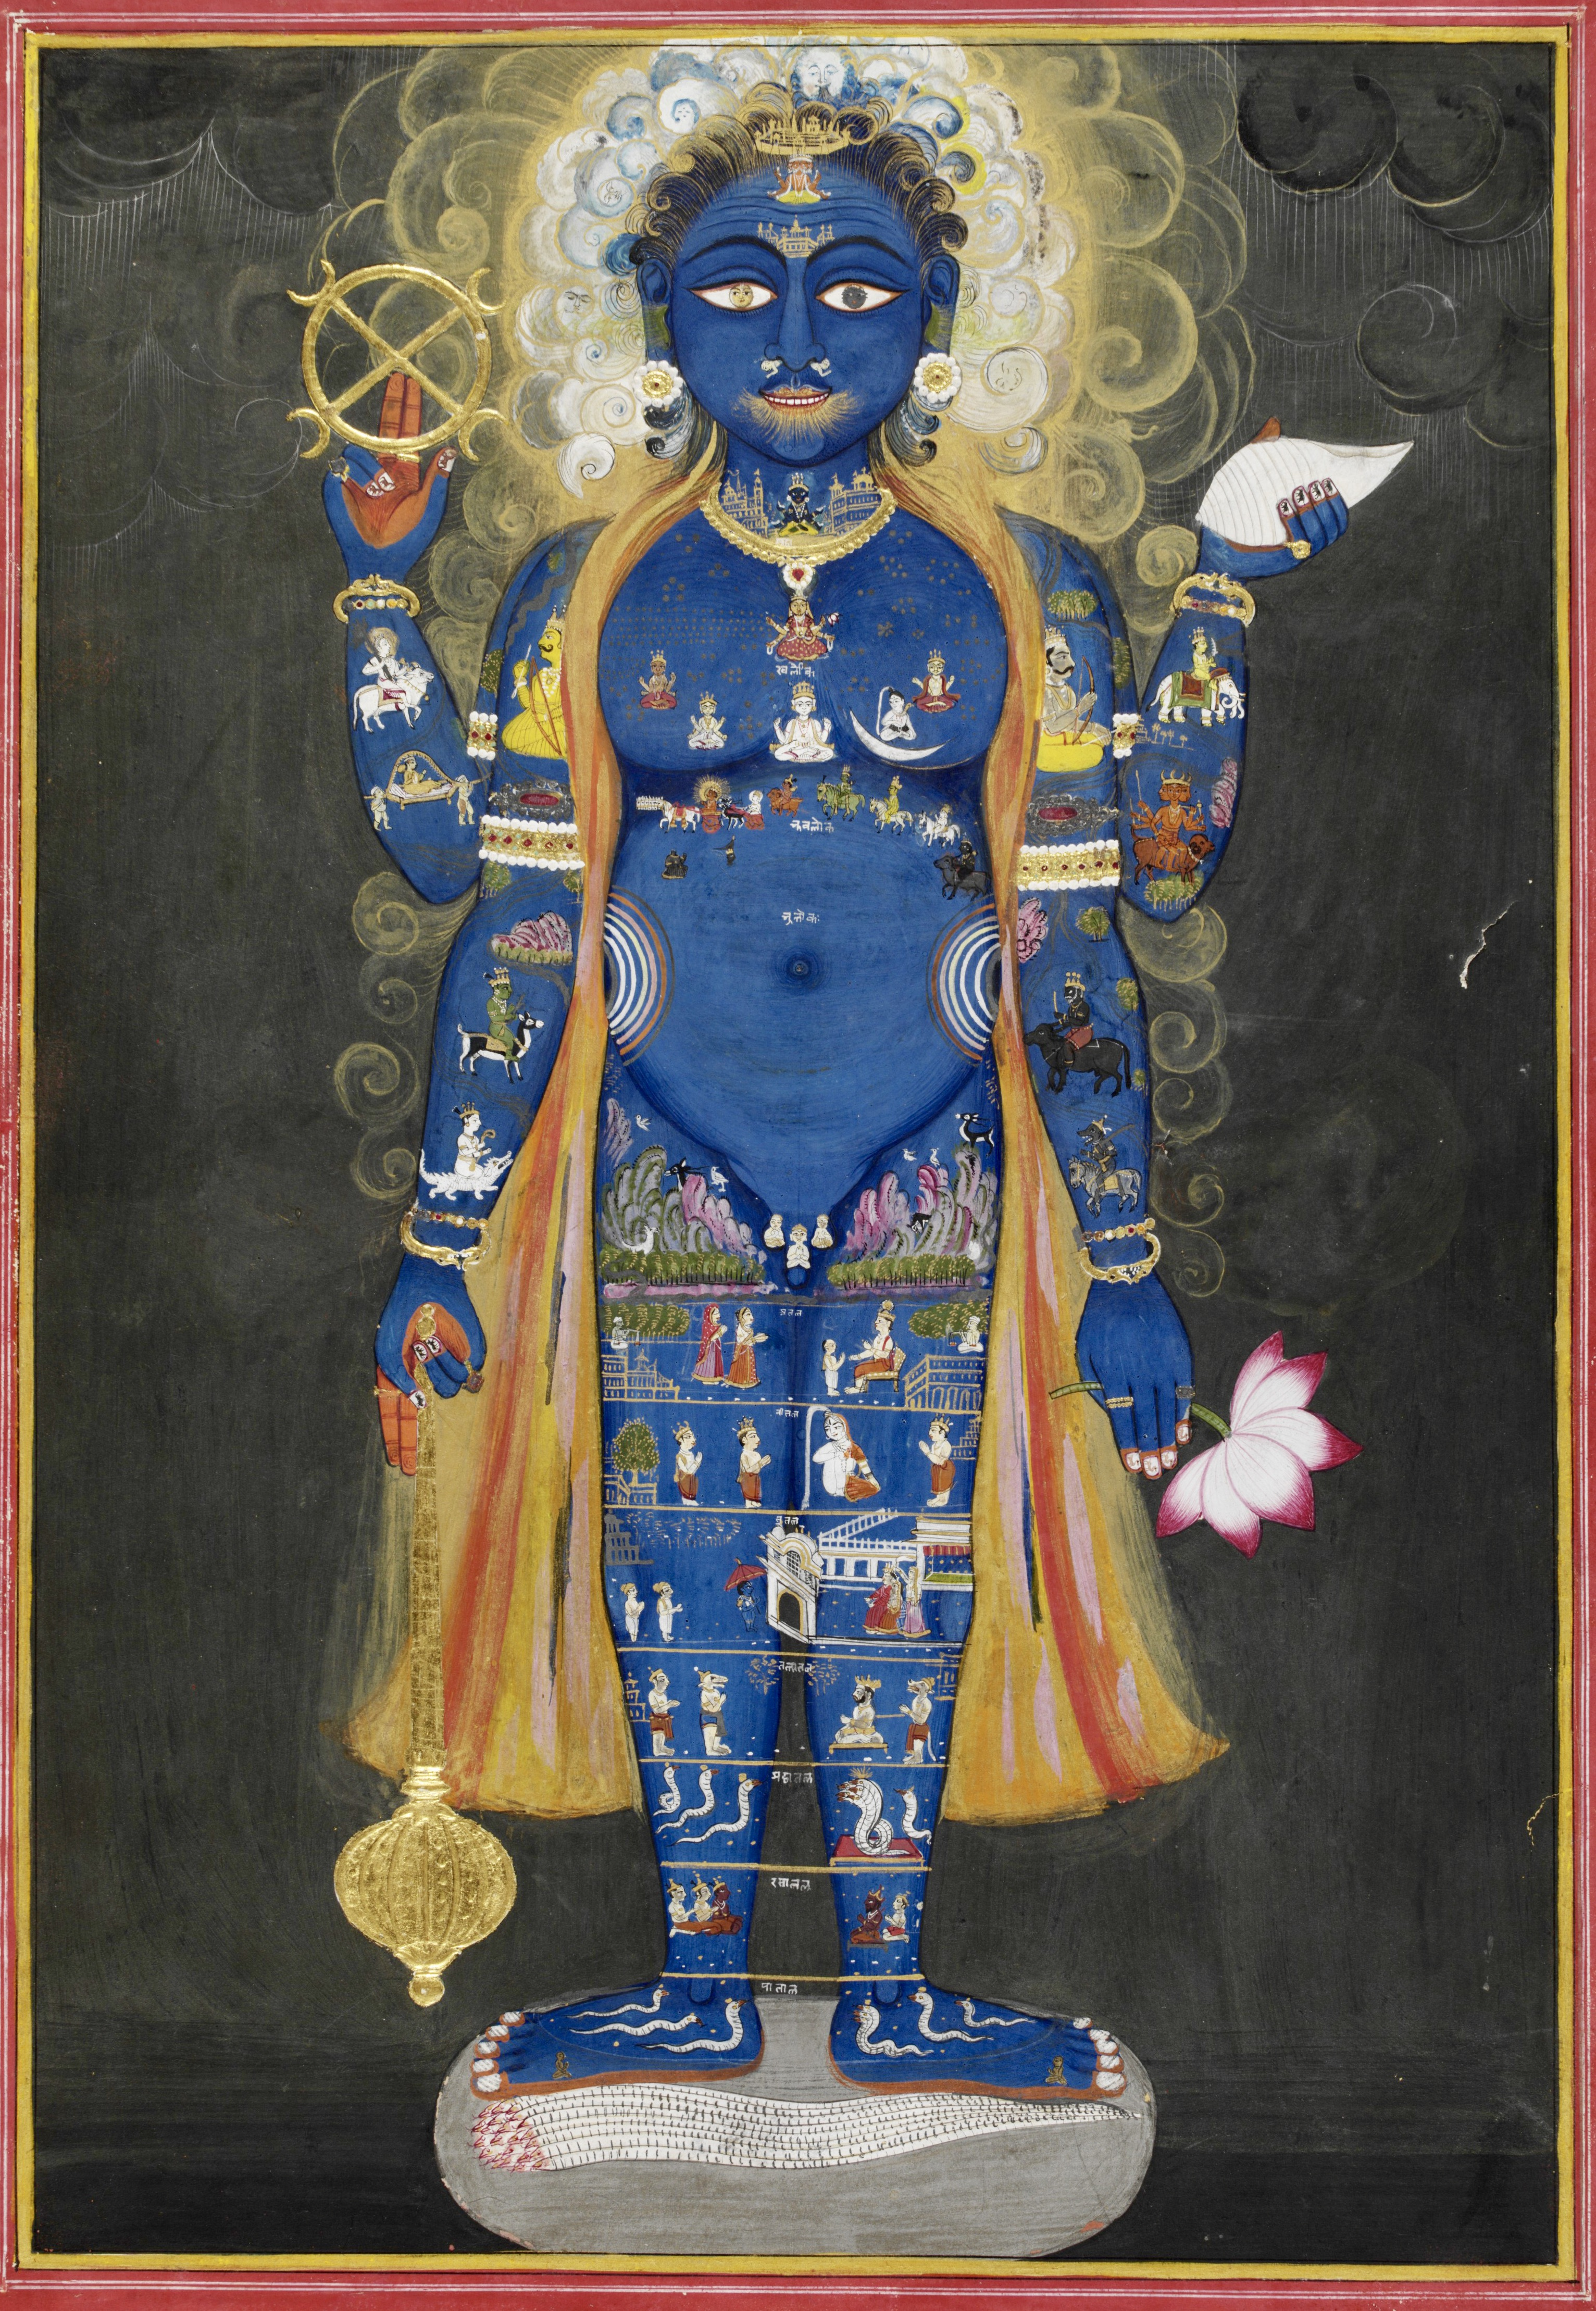
\includegraphics[width=1\textwidth]{pics/Vishnu_Vishvarupa_cropped.jpg}
	\caption{Viṣṇu Viśvarūpa, India, Rajasthan, Jaipur, ca. 1800–1820, Opaque watercolor and gold on paper, 38.5 × 28 cm, Victoria and Albert Museum, London, Given by Mrs. Gerald Clark.}
	\label{fig1}
      \end{figure}
\clearpage
  \begin{figure}[ht]
	\centering
  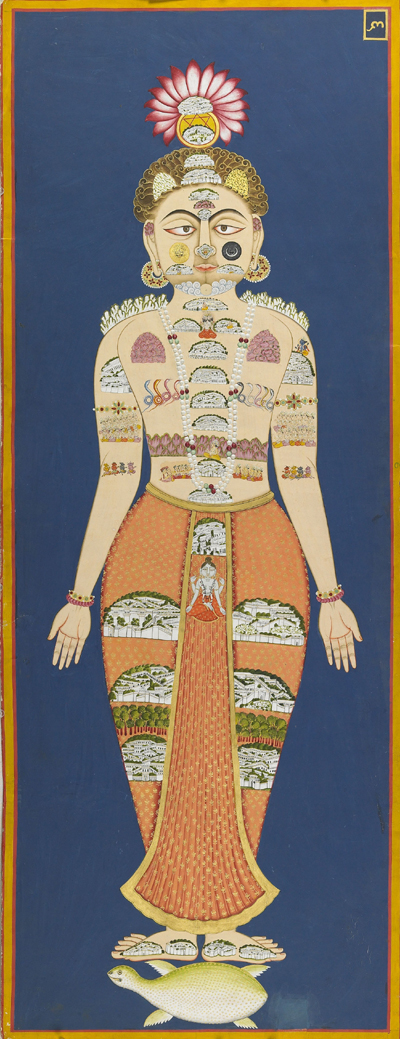
\includegraphics[width=0.5\textwidth]{pics/The_Equivalence_of_Self_and_Universe_(detail),_folio_6_from_the_Siddha_Siddhanta_Paddhati,_(Bulaki),_1824_(Samvat_1881);_122_x_46_cm._Mehrangarh_Museum_Trust..jpg}
	\caption{The Equivalence of Self and Universe (detail), folio 6 from the \textit{Siddhasiddhāntapaddhati} (Bulaki), India, Rajasthan, Jodhpur, 1824 (Samvat 1881), 122 x 46 cm, RJS 2378, Mehragarh Museum Trust.}
	\label{fig2}
      \end{figure}
      % \end{landscape}


\chapter{Bibliography}
 \label{sec:bibli}
   \clearpage
\newpage 
\thispagestyle{empty}
\quad  \addtocounter{page}{-1}

\printbibliography[heading=subbibintoc, title=Consulted Manuscripts, keyword=codex]

\printbibliography[heading=subbibintoc, title=Printed Editions, keyword=printsource]

\printbibliography[heading=subbibintoc, title=Secondary Literature, keyword=seclit]

\printbibliography[heading=subbibintoc, title=Online Sources, keyword=onlinesource]

\end{document}
